%! TeX program = lualatex
%% This is the ctufit-thesis example file. It is used to produce theses
%% for submission to Czech Technical University, Faculty of Information Technology.
%%
%% This is version 1.4.2, built 20. 3. 2025.
%%
%% Get the newest version from
%% https://gitlab.fit.cvut.cz/theses-templates/FITthesis-LaTeX
%%
%%
%% Copyright 2024, Tomas Novacek
%% Copyright 2021, Eliska Sestakova and Ondrej Guth
%%
%% This work may be distributed and/or modified under the
%% conditions of the LaTeX Project Public License, either version 1.3
%% of this license or (at your option) any later version.
%% The latest version of this license is in
%%  https://www.latex-project.org/lppl.txt
%% and version 1.3 or later is part of all distributions of LaTeX
%% version 2005/12/01 or later.
%%
%% This work has the LPPL maintenance status `maintained'.
%%
%% The current maintainer of this work is Tomas Novacek (novacto3@fit.cvut.cz).
%% Alternatively, submit bug reports to the tracker at
%% https://gitlab.fit.cvut.cz/theses-templates/FITthesis-LaTeX/issues
%%
%%

% arara: xelatex
% arara: biber
% arara: xelatex
% arara: xelatex

%%%%%%%%%%%%%%%%%%%%%%%%%%%%%%%%%%%%%%%%%
% CLASS OPTIONS
% language: czech/english/slovak
% thesis type: bachelor/master/dissertation
% colour: bw for black&white OR no option for default colour scheme
% electronic (oneside) or printed (twoside), twoside is default
% paragraph - if passed, this optional argument sets paragraphs as the deepest level of headers, styles it, numbers it and adds it to Table of Content. Use with care! Normally, it is considered unwise to use it, since its too deep.
%%%%%%%%%%%%%%%%%%%%%%%%%%%%%%%%%%%%%%%%%
\documentclass[english,master,twoside]{ctufit-thesis}

%%%%%%%%%%%%%%%%%%%%%%%%%%%%%%%%%%
% BASIC INFORMATION
%%%%%%%%%%%%%%%%%%%%%%%%%%%%%%%%%%
\ctufittitle{Understanding Feedback Pollution in the R Programming Language}
\ctufitauthorfull{Bc. Filip Říha}
\ctufitauthorsurnames{Říha}
\ctufitauthorgivennames{Filip}
\ctufitsupervisor{doc. Ing. Filip Křikava\, Ph.D.}
\ctufitdepartment{Department of Theoretical Computer Science}
\ctufityear{2025}
\ctufitdeclarationplace{Prague}
\ctufitdeclarationdate{\todo{\today}}

\ctufitabstractCZE{TODO}
\ctufitabstractENG{TODO}
\ctufitkeywordsCZE{TODO}
\ctufitkeywordsENG{TODO}
%%%%%%%%%%%%%%%%%%%%%%%%%%%%%%%%%%
% END BASIC INFORMATION
%%%%%%%%%%%%%%%%%%%%%%%%%%%%%%%%%%

%%%%%%%%%%%%%%%%%%%%%%%%%%%%%%%%%%
% CUSTOMIZATION of this template
%%%%%%%%%%%%%%%%%%%%%%%%%%%%%%%%%%
\RequirePackage{iftex}[2020/03/06]
\iftutex % XeLaTeX and LuaLaTeX
    \RequirePackage{ellipsis}[2020/05/22] %ellipsis workaround for XeLaTeX
\else
    \errmessage{Only compilation with XeLaTeX or LuaLaTeX is allowed}
    \stop
\fi

% hyperlinks
\hypersetup{
    pdfpagelayout=TwoPageRight,
    colorlinks=false,
    allcolors=decoration,
    pdfborder={0 0 0.1}
}

% change the colour of all hyperlinks to CTU blue
\hypersetup{allbordercolors=decoration}

\RequirePackage{pdfpages}[2020/01/28]

%%%%%%%%%%%%%%%%%%%%%%%%%%%%%%%%%%
% CUSTOMIZATION of this template END
%%%%%%%%%%%%%%%%%%%%%%%%%%%%%%%%%%


%%%%%%%%%%%%%%%%%%%%%%
% PACKAGES SETTINGS
%%%%%%%%%%%%%%%%%%%%%%
\usepackage{dirtree}
\usepackage{tikz}
\usepackage[style=iso-numeric]{biblatex}
\addbibresource{text/bib-database.bib}
\usepackage{xurl}

\usepackage{subcaption}
\renewcommand{\thesubtable}{\thetable.\arabic{subtable}}

\usepackage[newfloat]{minted}
\SetupFloatingEnvironment{listing}{name=Code listing}
\DeclareCaptionSubType*[arabic]{listing}
\setminted{linenos}
\newcommand{\mintoneline}[2]{\mint[linenos=false]{#1}{#2}}

\usepackage{calc}

\usepackage{csquotes}
\newcommand{\quotecite}[1]{\enquote{\textit{#1}}}

\newcommand{\todo}[1]{\textbf{\textcolor{red}{(TODO: #1)}}}
\newcommand{\todoadd}[0]{\textbf{\textcolor{red}{(TODO)}}}
\newcommand{\todocite}[0]{[\textbf{\textcolor{red}{?}}]}

\usepackage{multirow}

% Custom commands
\newcommand{\SEXP}[0]{\texttt{SEXP}}

%%%%%%%%%%%%%%%%%%%%%%
% PACKAGES SETTINGS END
%%%%%%%%%%%%%%%%%%%%%%

\begin{document}
\frontmatter\frontmatterinit % do not remove these two commands

\thispagestyle{empty}\maketitle\thispagestyle{empty}\cleardoublepage % do not remove these four commands

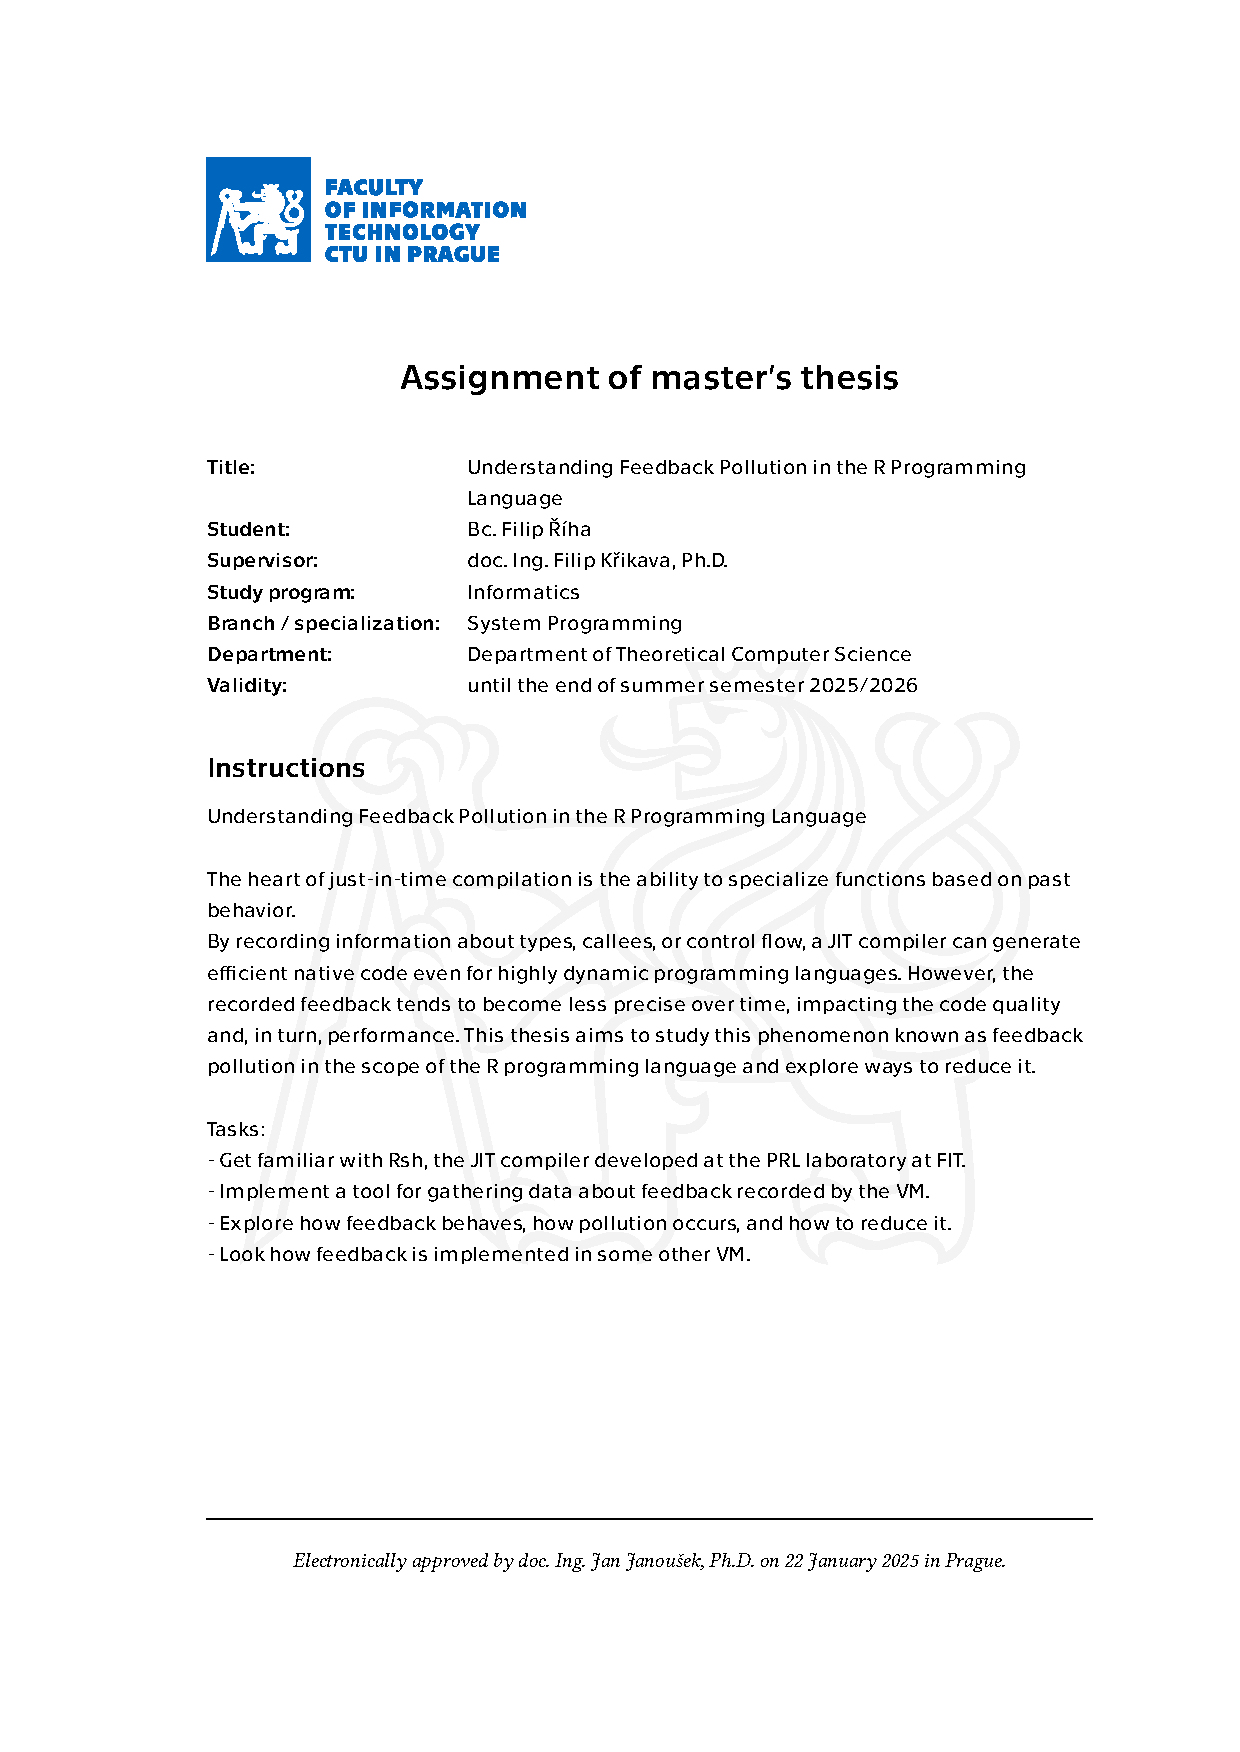
\includepdf[pages={1-}]{rihafili-assignment.pdf}

\imprintpage % do not remove this command
\stopTOCentries
%%%%%%%%%%%%%%%%%%%%%%
% list of other contents END
%%%%%%%%%%%%%%%%%%%%%%

%%%%%%%%%%%%%%%%%%%
% ACKNOWLEDGMENT
%%%%%%%%%%%%%%%%%%%
\begin{acknowledgmentpage}
	\todoadd
\end{acknowledgmentpage}
%%%%%%%%%%%%%%%%%%%
% ACKNOWLEDGMENT END
%%%%%%%%%%%%%%%%%%%


%%%%%%%%%%%%%%%%%%%
% DECLARATION
% FILL IN / MODIFY
%%%%%%%%%%%%%%%%%%%
\begin{declarationpage}
	\todo{is this the correct declaration (should be for GPL)}
	I hereby declare that the presented thesis is my own work and that I have cited all
	sources of information in accordance with the Guideline for adhering to ethical
	principles when elaborating an academic final thesis.

	I acknowledge that my thesis is subject to the rights and obligations stipulated by the
	Act No. 121/2000 Coll., the Copyright Act, as amended. In accordance with Article 46 (6)
	of the Act, I hereby grant a nonexclusive authorization (license) to utilize this thesis,
	including any and all computer programs incorporated therein or attached thereto and
	all corresponding documentation (hereinafter collectively referred to as the “Work”), to
	any and all persons that wish to utilize the Work. Such persons are entitled to use the
	Work for non-profit purposes only, in any way that does not detract from its value. This
	authorization is not limited in terms of time, location and quantity.
\end{declarationpage}
%%%%%%%%%%%%%%%%%%%
% DECLARATION END
%%%%%%%%%%%%%%%%%%%

\printabstractpage

%%%%%%%%%%%%%%%%%%%%%%
% list of contents
%%%%%%%%%%%%%%%%%%%%%%
\tableofcontents

\listoffigures
\begingroup
\let\clearpage\relax
\listoftables
\thectufitlistingscommand
\endgroup
%%%%%%%%%%%%%%%%%%%%%%
% list of contents END
%%%%%%%%%%%%%%%%%%%%%%

%%%%%%%%%%%%%%%%%%%
% ABBREVIATIONS
% List the abbreviations in lexicography order.
%%%%%%%%%%%%%%%%%%%
\chapter{\thectufitabbreviationlabel}

\begin{tabular}{rl}
	AST  & Abstract Syntax Tree        \\
	GC   & Garbage Collector           \\
	IR   & Intermediate Representation \\
	JIT  & Just-in-time                \\
	OSR  & On-Stack Replacement        \\
	SSA  & Static Single-Assignment    \\
	SEXP & Symbolic Expression         \\
	VM   & Virtual Machine             \\
\end{tabular}
%%%%%%%%%%%%%%%%%%%
% ABBREVIATIONS END
%%%%%%%%%%%%%%%%%%%

%%%%%%%%%%%%%%%%%%%
% THE THESIS
%%%%%%%%%%%%%%%%%%%

\resumeTOCentries
\mainmatter\mainmatterinit % do not remove these two commands

%---------------------------------------------------------------
\chapter*{Introduction}\addcontentsline{toc}{chapter}{Introduction}\markboth{Introduction}{Introduction}
%---------------------------------------------------------------
\setcounter{page}{1}

Many modern dynamic languages are executed on a virtual machine (VM). In order to speed up the execution of programs, VMs traditionally include a Just-in-Time (JIT) compilers, allowing them to improve the performance of frequently executed pieces of programs by compiling them to native code. To further enhance the performance, most modern VMs record information about the runtime (called feedback), allowing them to predict future behaviour and optimize the compilation even more, resulting in faster execution. This is based on the thesis that what is past is prologue. However, over time, the recorded information tends to become less precise, resulting in more general assumptions and slower code down the line. This trend is known as feedback pollution.

R is a high-level programming language specialized for statistical computing and data visualization. It is dynamically typed with function and object-oriented patterns, and supports reflection and lazy evaluation. GNU-R, the de-facto reference implementation of R, contains both an abstract syntax tree (AST) interpreter and a bytecode JIT compiler and interpreter, but the compiler is not speculative. Ř is an alternative JIT compiler for GNU-R. It uses feedback information from an interpreter to speculatively optimize the native compilation. However, the inner workings of Ř are sort of a black box, as there is no simple way to trace its functionality.

The main goal of this thesis is to implement a tool that would allow us to observe and analyze the behavior of the Ř compiler, allowing us to better understand the Ř internals and opening up possibilities for further research and analysis. One of these research paths is the amount and impact of the feedback pollution as it happens in R.

In chapter 1, we introduce the necessary background information, including the R language, GNU-R virtual machine implementation, and the Ř compiler structure. Chapter 2 delves into the design and implementation of the recording tool, as well as its impact on the Ř codebase. Chapter 3 outlines the research done on the feedback pollution, which was possible thanks to the recording tool. Chapter 4 then further analyzes how the feedback information is used (or not used) during compilation, observing feedback patterns in the compiler and connecting them to the feedback pollution.


%---------------------------------------------------------------
\chapter{Background}
%---------------------------------------------------------------

\begin{chapterabstract}
	\todoadd
\end{chapterabstract}

%------------------------------------------------------------------------------------------------------------------------------
\section{The R Language}
%------------------------------------------------------------------------------------------------------------------------------

\textit{R}\cite{r} is a programming language used for statistical computation and data visualization. It was developed Ross Ihaka and Robert Gentleman at the University of Auckland as an alternative to the S language. It is part of the GNU Project, licensed as a free software under GNU GPL.

The beauty of R is that very complex operations can be expressed in very few lines of code, as demonstrated in listing \ref{lst:motivation}. It is used a lot by statistician, where a big part of them are non-programmers, and this is reflected in the design of the language. It allows for high levels of abstractions, expressive domain-specific languages and APIs and code that is very \todoadd

\begin{figure}[hb]
	\centering
	\begin{minipage}{0.45\textwidth}
		\centering
		\begin{minted}{R}
ggplot(
  data = gapminder,
  aes(
    x = gdpPercap, y = lifeExp,
    color = continent
  )
) +
  geom_point() +
  scale_x_log10()
      \end{minted}
		\captionof{listing}{R example\todocite}\label{lst:motivation}
	\end{minipage}%
	\hfill
	\begin{minipage}{0.45\textwidth}
		\centering
		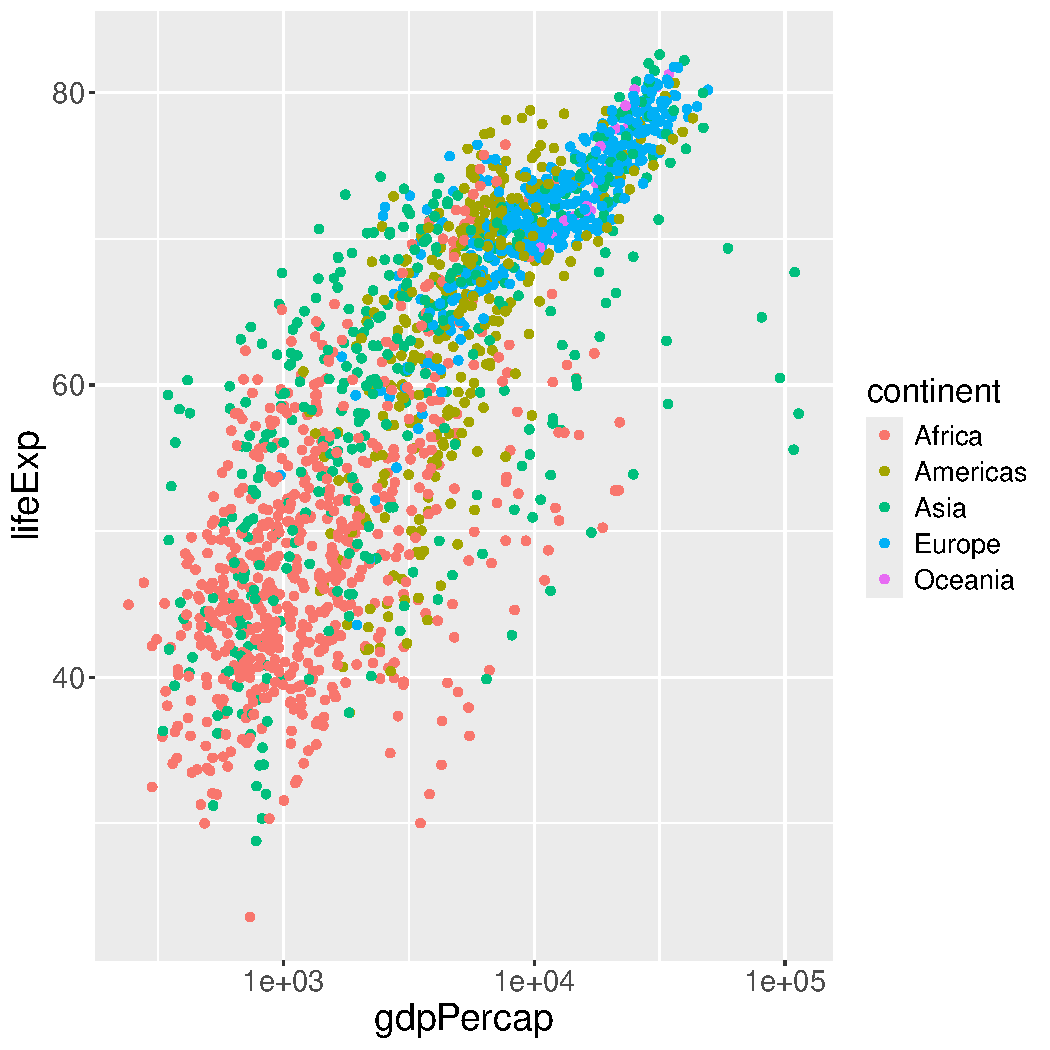
\includegraphics[width=\textwidth]{figures/motivation-Rplots.pdf}
		\caption{Plot of listing \ref{lst:motivation}}
	\end{minipage}
\end{figure}

\newpage
The language is high-level, dynamic, object-oriented, functional, interpreted, and lazy, with automatic memory management.

The R syntax is very C-like, with \texttt{if} statements, \texttt{for} and \texttt{while} loops, array indexing and function calls. For assignment, the \texttt{<-} operator is used. Statements are separated by newline, optionally by semicolon if they are on the same line.

%---------------------------------------------------------------
\subsubsection*{Types}
%---------------------------------------------------------------

R basic types are the \textit{numeric types} (\textit{integer}, \textit{double} or also \textit{real} and \textit{complex}), \textit{character type} (strings) and \textit{logical type} (the boolean values \texttt{TRUE} and \texttt{FALSE}). R also has \texttt{NULL}, and a constant \texttt{NA} (\textit{not available}) representing a missing value.

R has no concept of scalars. Instead, all basic types are represented as \textit{vectors}. To create a vector with multiple elements, the function \texttt{c} (standing for combine) can be used. All the traditional mathematical operators are also vectorized.

For storing elements of different types, a \textit{list} is used. Other commonly used types built on top of vectors and lists are \textit{matrix} (two-dimensional vector), \textit{array} (multi-dimensional vector) and \textit{data frame} (matrix-like structure whose columns can have different types).

Every type can have associated \textit{attributes}, a collection of name-value pairs. These are accessed via the \texttt{attr} or \texttt{attributes} functions.

R also has multiple \textit{object models}. The most common ones are \textit{S3}, which is controlled by setting a \texttt{class} attribute on any type, and \textit{S4}, which defines more formal classes which have to be created and instantiated, and are internally represnted by a distinct type.

%---------------------------------------------------------------
\subsubsection*{Environments}
%---------------------------------------------------------------

Different scopes in R are separated using objects named \textit{environments}. An environment consists of a \textit{frame}, which is the collection of variables, and a pointer to an \textit{enclosing environment} (also called a \textit{parent}). The topmost environment has a pointer to a special \textit{empty environment}, which has no other parent.

When a variable or a function is accessed, it is first looked for in the current environment. If not found, it is searched for recursively in each enclosing environment. Only then if it is not found, it is an error.

The lookup for functions is separate from non-function lookup. An assignment of a variable in some environment does not shadow a function in its enclosing environment. So the code \texttt{c <- 42; c(c, c)} results in one vector with two numbers 42, because the definition of the variable \texttt{c} does not shadow the function of the same name from the base environment.

These environments are also first-class values. We can create new environments, access the value of the current enclosing environment, or even access and modify environments on the call stack.

%---------------------------------------------------------------
\subsubsection*{Functions}
%---------------------------------------------------------------

A \textit{function}, or also a \textit{closure}, is composed of three parts - \textit{formals}, which is the list of formal arguments and their default values, \textit{body}, which is the code of the function, and \textit{environment} defining the lexical scope of the function body. New functions can be created with the \texttt{function} keyword.

Most operations that happen in R are in fact function calls. This includes the control flow statements (like \textit{if} or \textit{while}), binary operations, assignment, and even surrounding an expression with parenthesis or multiple expression with braces. This is demonstrated in listing \ref{lst:r-special-calls}. Note that built-in functions have to be surrounded with backticks in order to referr to them as identifiers.

\begin{listing}[t]
	\begin{sublisting}[t!]{0.47\textwidth}
		\centering
		\begin{minted}{R}
a <- if (TRUE) {
  1
} else
  2 * (3 + 4)
    \end{minted}
	\end{sublisting}
	\hfill
	\begin{sublisting}[t!]{0.47\textwidth}
		\centering
		\begin{minted}{R}
# This is equivalent to
# the previous statement
`<-`(a, `if`(
  TRUE,
  `{`(1),
  `*`(
    2,
    `(`(`+`(3, 4))
  )
))
    \end{minted}
	\end{sublisting}
	\caption{Demonstration of R special calls}\label{lst:r-special-calls}
\end{listing}

%---------------------------------------------------------------
\subsubsection*{Laziness}
%---------------------------------------------------------------

R is lazy in arguments. This means that when a function is called, the passed arguments are not instantly evaluated, but are instead wrapped in a \textit{promise}, a tuple of \textit{expression}, \textit{value}, and \textit{environment}. The value is at first set to the unbound value. When the promise is first accessed, the expression of the promise is evaluated with its environment (also called a \textit{force}). The result is cached in the value field, and every other access to the argument results in the cached value.

This can be seen in example \ref{lst:example-lazy}. The call at line 12 first prints \enquote{Hello from g}, then the parameter \texttt{x} is accessed, the promise is forced, and the text \enquote{Hello from f} is printed. The second call to the function \texttt{h} demonstrates a second behavior - when a parameter is never accessed, the promise is not evaluated, and nothing is printed.

\begin{listing}[h!]
	\centering
	\begin{minted}{R}
f <- function(x) {
    print("Hello from f")
    x
}

g <- function(x) {
    print("Hello from g")
    x
}

# Prints "Hello from g", then "Hello from f"
g(f(42))

h <- function(x) 0

# Does not print anything
h(f(42))
  \end{minted}
	\caption{Example of R laziness}\label{lst:example-lazy}
\end{listing}

Being lazy in the arguments allows R to have very expressive domain-specific languages for ease of manipulating the data, as well as reducing memory overhead of the programs.

Promises can also be created manually by calling the \texttt{delayedAssign} function or from the C API.

%---------------------------------------------------------------
\subsubsection*{Immutability}
%---------------------------------------------------------------

All R values are \textit{semantically immutable}, with the exception of environments. This means that when a variable holds a value, this value never changes unless the variable is reassigned. We say that non-environment values have a \textit{copy-on-write behavior} - when a value is modified, a new copy is created with the modified parts.

Thanks to the syntax of R, it is possible to write code that looks like it is using mutability, but keeps the copy-on-write behavior. In the example \ref{lst:imm}, the statement on line 3 looks like it is mutating the vector in place, but instead the function \texttt{[<-} is called, which creates a copy of the vector, modifies it and reassigns the variable x.

The only truly mutable values are environments, and they conform to a \textit{reference behavior}. Listing \ref{lst:envir} shows this behavior - the variable \texttt{x} is added to both \texttt{e1} and \texttt{e1}, even though we only defined it on \texttt{e2}.

\begin{listing}
	\centering
	\begin{minipage}{0.47\textwidth}
		\begin{minted}{R}
x <- c(1, 2, 3)
y <- x
y[1] <- 42
# x is still vector (1, 2, 3)
      \end{minted}
		\caption{Immutability example}\label{lst:imm}
	\end{minipage}
	\hfill
	\begin{minipage}{0.47\textwidth}
		\begin{minted}{R}
e1 <- new.env()
e2 <- e1
e2$x <- 42
e1$x == 42
# TRUE
      \end{minted}
		\caption{Example of environment mutability}\label{lst:envir}
	\end{minipage}
\end{listing}

%---------------------------------------------------------------
\subsubsection*{Reflection}
%---------------------------------------------------------------

As mentioned before, environments are a first-class citizen. This allows for any function to access and even modify any environment where it was created or called. Moreover, when combined with lazy arguments, a function can reflect on the environment it is being forced in and modify it, sometimes in unpredictable ways.

This is demonstrated in listing \ref{lst:bad-ref}, where we call to \texttt{good}, inside of which we evaluate to the call to \texttt{bad}, which reflects on the caller environment, deletes a binding, and results in a unbinded variable on line 9.\todo{rewrite}

\begin{listing}
	\centering
	\begin{minted}{R}
bad <- function() {
  rm("x", envir=sys.frame(-1)) # Remove the variable x from the caller
  2
}

good <- function(y) {
  x <- 1
  z <- y # Here the promise is evalated
  x + z
}

good(bad())
# Error in good(bad()) : object 'x' not found
  \end{minted}
	\caption{Example of malicious reflection\todocite}\label{lst:bad-ref}
\end{listing}

R also has primitives for creating, manipulating, and evaluating expressions from the language itself. This allows for, among other things, evaluate a promise under a different environment, programatically create arbitrary pieces of code, or instrument functions with additional calls \todo{different example \dots}.

Combining reflection, laziness and side effects makes R a very complex language to optimize.

\newpage
%------------------------------------------------------------------------------------------------------------------------------
\section{GNU-R}
%------------------------------------------------------------------------------------------------------------------------------

The R language is not formally specified, it only has a reference implementation that we will refer to as \textit{GNU-R}\todocite. It is written in the C programming language, spans over more than {250 000} lines of code and is currently maintained by the R Core Team

%---------------------------------------------------------------
\subsubsection*{Representation}
%---------------------------------------------------------------

\todo{the attributes}
The GNU-R represents all code and values as \textit{symbolic expressions} (also \textit{S-expressions} or \textit{SEXPs}), a format for nested lists popularized by the Lisp languages. The type \texttt{SEXP} is a pointer to either a \texttt{SEXPREC} or \texttt{VECTOR\_SEXPREC} structure. Both of these structures contain a header of type \texttt{sxpinfo\_struct}, a pointer to the attributes of the current value, and previous and next nodes in the garbage collector. The header then contains \texttt{SEXPTYPE}, the type of the SEXP (values are defined as in \ref{tbl:sexptype}), as well as additional attributes with information about the type, garbage collection and debug information. The rest of the structure cointains the actual data. The structure of a \texttt{SEXP} value is represented in figure \ref{fig:sexp-struct}.

\begin{figure}
	\centering
	\begin{adjustbox}{trim=5pt 20pt 0 40pt, clip}
		\includediagram{0}
	\end{adjustbox}
	\caption{Structure of the GNU-R \texttt{SEXP} type}\label{fig:sexp-struct}
\end{figure}

\begin{table}[h!]
	\begin{tabular}{c l l}
		\textbf{no} & \textbf{SEXPTYPE} & \textbf{Description}       \\
		\hline
		0           & NILSXP            & NULL                       \\
		1           & SYMSXP            & symbols                    \\
		2           & LISTSXP           & pairlists                  \\
		3           & CLOSXP            & closures                   \\
		4           & ENVSXP            & environments               \\
		5           & PROMSXP           & promises                   \\
		6           & LANGSXP           & language objects           \\
		7           & SPECIALSXP        & special functions          \\
		8           & BUILTINSXP        & builtin functions          \\
		9           & CHARSXP           & internal character strings \\
		10          & LGLSXP            & logical vectors            \\
		13          & INTSXP            & integer vectors            \\
		14          & REALSXP           & numeric vectors            \\
		15          & CPLXSXP           & complex vectors            \\
		16          & STRSXP            & character vectors          \\
		17          & DOTSXP            & dot-dot-dot object         \\
		18          & ANYSXP            & make “any” args work       \\
		19          & VECSXP            & list (generic vector)      \\
		20          & EXPRSXP           & expression vector          \\
		21          & BCODESXP          & byte code                  \\
		22          & EXTPTRSXP         & external pointer           \\
		23          & WEAKREFSXP        & weak reference             \\
		24          & RAWSXP            & raw vector                 \\
		25          & OBJSXP            & objects not of simple type \\
	\end{tabular}
	\caption{The different SEXP types\cite[1.1.1 SEXPTYPEs]{rprojectInternals}}\label{tbl:sexptype}
\end{table}

%---------------------------------------------------------------
\subsubsection*{Interpreter}
%---------------------------------------------------------------

The GNU-R parses the code to an \textit{abstract syntaxt tree} (\textit{AST}), also represented with \texttt{SEXP}s with the \texttt{LANGSXP} type. \todo{interprets the tree}

After the first execution of a function or by calling \texttt{compiler::cmpfun} on it, the function is passed to a \textit{bytecode compiler}, written mostly in R with few supporting functions written in C. The bytecode is stack-based with fat instructions, like specialized instructions for type checking, specialized loads for common constants like \texttt{NULL}, \texttt{TRUE} or \texttt{FALSE}, instructions for executing \texttt{for} loops or various subsetting operators. Branching is done via jumps to arbitrary bytecode. An example of the bytecode can be seen in listing \ref{lst:bc-example-gnur}.

The bytecode employs a series of optimizations, most notably constant folding and inlining of base functions. The inlining can be set to various levels, with higher levels being more optimized while assuming that the functions in the base package and core language functions (like \texttt{if} or \texttt{`\{`}) are not shadowed. This allows the compiler to translate control flow from function calls to bytecode jumps, as well as to use bytecode instructions to perform basic arithmetic and logical operations.

When a function is compiled, its \texttt{SEXP} is modified in-place, replacing the AST body with a bytecode. Every other call to this function is then interpreted by the bytecode interpreter, which is written in C and is also is part of the GNU-R.

\begin{listing}[p]
	\centering
	\begin{minipage}{0.33\textwidth}
    \begin{minted}[fontsize=\small,linenos=false]{R}
f <- function(x) {
  for (i in 1:10) {
    if (i + 2 > 1) {
      g(x)
    }
  }
  g(x)
}
    \end{minted}
		\subcaption{R code}\label{lst:bc-example-r}
	\end{minipage}
	\hfill
	\begin{minipage}{0.66\textwidth}
		\begin{minipage}{0.20\textwidth}
			\begin{minted}[fontsize=\small,linenos=false]{text}
Code:
  1 LDCONST 1
  3 STARTFOR 4 3 30
  7 GETVAR 3
  9 LDCONST 5
 11 ADD 6
 13 LDCONST 7
 15 GT 8
 17 BRIFNOT 9 28
 20 GETFUN 10
 22 MAKEPROM 12
 24 CALL 11
 26 GOTO 29
 28 LDNULL
 29 POP
 30 STEPFOR 7
 32 ENDFOR
 33 POP
 34 GETFUN 10
 36 MAKEPROM 12
 38 CALL 11
 40 RETURN
      \end{minted}
		\end{minipage}
		\hfill
		\begin{minipage}{0.48\textwidth}
			\begin{minted}[fontsize=\small,linenos=false]{text}
Constant pool:
0:
 language {  for (i in 1:10) {; i..
1:
 int [1:10] 1 2 3 4 5 6 7 8 9 10
2:
 language 1:10
...
12:
 Promise 0:
  Code:
    1 GETVAR 0
    3 RETURN
  Constant pool:
  0:
   symbol x
  1:
   language g(x)
  2:
   'expressionsIndex' int [1:4] N..
13:
 'expressionsIndex' int [1:41] NA..
      \end{minted}
		\end{minipage}
		\subcaption{GNU-R code}\label{lst:bc-example-gnur}
	\end{minipage}
	\par\vspace{2mm}\par
	\begin{minipage}{\textwidth}
		\centering
		\begin{minipage}{0.47\textwidth}
			\begin{minted}[fontsize=\small,linenos=false]{\rirlexer}
0:
      0   push_  1
      5   visible_
      6   force_
      7   push_  10
     12   visible_
     13   force_
     14   ; :(1, 10)
          colon_input_effects_
     15   pop_
     16   swap_
     17   colon_cast_lhs_
     18   [ <?> ] Type#0
     23   ensure_named_
     24   swap_
     25   colon_cast_rhs_
     26   ensure_named_
     27   [ <?> ] Type#1
     32   dup2_
     33   ; NULL
          le_
     34   [ _ ] Test#0
     39   brfalse_  1
     44   push_  1L
     49   br_  2
      \end{minted}
		\end{minipage}
		\hfill
		\begin{minipage}{0.47\textwidth}
			\begin{minted}[fontsize=\small,linenos=false]{\rirlexer}
1:
     54   push_  -1L
     ...
7:
    287   popn_  3
    292   ldfun_  g
    297   [ 0, <0>, valid  ] Call#2
    302   mk_promise_  2
    307   ; g(x)
          call_  1
    324   [ <?> ] Type#11
    329   ret_

[Prom (index 0)]
0:
      0   ldvar_  x
      5   [ <?> ] Type#5
     10   ret_

[Prom (index 1)]
0:
      0   ldvar_  x
      5   [ <?> ] Type#9
     10   ret_
     ...
      \end{minted}
		\end{minipage}
		\subcaption{RIR code}\label{lst:bc-example-rir}
	\end{minipage}
  \caption{A truncated example of generated GNU-R and RIR bytecodes, full code in appendix \todoadd}\label{lst:bc-example}
% \ref{ch:appendix-bc}
\end{listing}


%---------------------------------------------------------------
\subsubsection*{Garbage Collector}
%---------------------------------------------------------------
R does not have primitives for managing memory, instead an automatic memory management provided by the runtime is expected. GNU-R uses a generational non-moving stop-the-world garbage collector with three generations\cite{r-gc-notes}.

Next to the GC, GNU-R also has a reference counter for each object, included in the object header. This is used for optimistic mutations - when an object would be copied and mutated, but there is only one reference to it, it is instead mutated in place, avoiding an unnecesarry copy. This correctly preserves the copy-on-write behavior.

%---------------------------------------------------------------
\subsubsection*{Packages}
%---------------------------------------------------------------

A big advantage of using R is the vast library of packages, libraries and data sets. These are hosted at \textit{The Comprehensive R Archive Network}\todocite package repository, wich is currated and tested by the R Core Team. They can be very simply installed by calling \texttt{install.packages} and loaded with the \texttt{library} function.

The GNU-R base installation is also distributes with several packages, including, but not limited to, \texttt{base} containing the basic functions for using R, \texttt{stats} implementing statistical functions, \texttt{graphics} with base functions for manipulating graphical output, \texttt{compiler} implementing the mentioned bytecode compiler, or \texttt{Matrix} with hiearchy of dense and sparse matrix classes.

%---------------------------------------------------------------
\subsubsection*{C interface}
%---------------------------------------------------------------

In order to speed-up certain packages, GNU-R allows parts of the code to be written in more low-level languages via a C interface. This includes the definitions for the SEXP types, a big set of functions and macros to create and manipulate values, as well as several evaluations functions. The SEXP structure is only exported as an opaque pointer, with the intent that individual fields are to be accessed and manipulated via the exported functions.

The interface is more of an after thought more than a deliberate choice, as indicated for example by the the main file with type definitions being called \texttt{Rinternals}. The functions expose big portion of the internal structure and this is subsequently used by package authors. Even parts of the code that are not directly exposed are commonly accessed by packages. As an example, some packages rely on the hidden reference counter in order to optimize updates by modifying structures in-place.

This makes evolution of R without breaking packages very hard, as well as complicating alternative implementations of R as they need to explicitly export the same functions as GNU-R if they want to support all available libraries.

\newpage
%------------------------------------------------------------------------------------------------------------------------------
\section{The Ř compiler}
%------------------------------------------------------------------------------------------------------------------------------

\textit{Ř} (also stylized as \textit{Rsh}) is a just-in-time compiler for the R language, developed at Programming Languages Laboratory at Czech Technical University in Prague\footnote{\url{https://prl-prg.github.io/}} and Programming Research Laboratory at Notheastern University\footnote{\url{https://prl.khoury.northeastern.edu/}}. The project is freely available and hosted on GitHub\todocite.

It is built as an extension to GNU-R, although it uses a slightly modified version of the codebase. It bypasses the GNU-R bytecode compiler and interpreter, instead using a custom one, while reusing the \texttt{SEXP} representation, AST interpreter, and garbage collector. For the compilation to native code, the \textit{LLVM Project}\cite{llvm} is used. The compilation pipeline is outlined in figure \ref{fig:rsh-archit}

\begin{figure}
	\centering
	\includediagram[0.7]{3}
	\caption{Overview of Ř architecture\cite{reusing-jit}}\label{fig:rsh-archit}
\end{figure}

%---------------------------------------------------------------
\subsubsection*{Runtime objects}
%---------------------------------------------------------------

Ř uses the GNU-R \texttt{SEXP} representation and memory management. All runtime objects are embedded into the SEXP objects. This is one of the modifications that need to be applied to GNU-R, a new \texttt{SEXPTYPE} is added (\texttt{EXTERNALSXP}), along with the necessary changes to how it is garbage collected and how it references other objects.

The structure of Ř runtime object can be seen in figure \ref{fig:rsh-object-struct}. It represented as the \texttt{SEXP} header, the \texttt{SEXPTYPE} alwyas set to the \texttt{EXTERNALSXP}, and then the embeded \texttt{RirRuntimeObject}. This object always starts with two \texttt{uint32\_t} numbers, the first dictates how many bytes after the start of the Ř object do start the pointers to the other \texttt{SEXP}s, and the second indicates how many pointers are there. The magic number dictates which Ř object it is.

There are helpers macros to access the headers, as well as the pointers to other \texttt{SEXP}s. On the Ř side, there are functions to convert between a C++ pointer and a SEXP.

\begin{figure}
	\centering
	\begin{adjustbox}{trim=10 80pt 0 0, clip}
		\includediagram{1}
	\end{adjustbox}
	\caption{Structure of the Ř runtime objects}\label{fig:rsh-object-struct}
\end{figure}

Similarly to the GNU-R compiler, when an R function is to be interpreted, it is compiled to a bytecode, and the body field of the closure is instead replaced by a Ř structure. The composition of Ř objects can be seen in figure \ref{fig:rsh-composition}.

The body of Ř compiled function contains a \textit{dispatch table}. A dispatch table contains multiple entries of compiled code, where the first version (also called a \textit{baseline}) is always the bytecode representation, whereas the other versions are compiled to native code. Each native entry corresponds to one context for contextual dispatch (explained in chapter \ref{ch:1-ctx-dispatch}).

Every dispatch table entry is represented by a \texttt{Function} structure. This holds the signature of the function, the context for contextual dispatch, statistic about the execution like how many times it has been invoked or deopted, the body of the function and the feedback vector.

The body of a function is stored in a structure called \texttt{Code}. This is either the bytecode body or a pointer to the native function, and the constants pool.

The \textit{feedback vector} collected from a bytecode interpretation is represented by the \texttt{TypeFeedback} structure\footnote{\texttt{TypeFeedback} is a missleading name as the interpreter also collect non-type information}. It consists of \textit{slots}, where one slot corresponds to information about one bytecode instruction, and there are three different types of slots. \textit{Observed calls} records the destination of calling a function, \textit{observed types} record the types of values that are loaded from environment, forced, or are results of a function call, and \textit{observed tests} has one of four values recording how a branch was taken (\texttt{None}, \texttt{OnlyFalse}, \texttt{OnlyTrue} and \texttt{Both}). Since every function has different number of slots, the \texttt{TypeFeedback} object has different size for each function and is using a \textit{flexible array member}\todocite to store the observed values.

\begin{figure}
	\centering
	\includediagram[0.7]{2}
	\caption{Composition of Ř runtime objects}\label{fig:rsh-composition}
\end{figure}

%---------------------------------------------------------------
\subsubsection*{RIR bytecode interpreter}
%---------------------------------------------------------------

The bytecode used by Ř is called \textit{RIR}. It is a stack-based bytecode, interpreted by a Ř interpreter. It uses the GNU-R bytecode execution stack. Unlike the GNU-R bytecode, the RIR instructions are much more granular, there are fewer of them, they are not as specialized and a single instruction represent much smaller piece of C code that in GNU-R. An example of RIR compiled code can be seen in listing \ref{lst:bc-example-rir}. Note that the example code is not complete and is only used to give impression between the size differences of the bytecodes. The full code listing is in appendix \todoadd.

For this thesis, the important bytecode instructions are \texttt{record\_call\_}, \texttt{record\_type\_}, and \texttt{record\_test\_}. These do the recording of feedback information about calls, types and tests respectively by observing the top value on the execution stack and recording the information to the \texttt{TypeFeedback} structure on an index stored as an immediate. The instructions are printed in listings as the observed values in square brackets followed by the label \texttt{Call\#N}, \texttt{Type\#N} or \texttt{Test\#N}, where \texttt{N} is the slot index.

Apart from the runtime values, the RIR interpreter also records other informations about the running program, most notably the number of times a function has been invoked, and the number of times a loop has been executed. These are used to determine which parts of the program are executed frequently, and thus are a good candidates for compiling to native code.

%---------------------------------------------------------------
\subsubsection*{PIR compiler}
%---------------------------------------------------------------
When a function or a loop meets the compilation heuristics, it is compiled to \textit{PIR}, an intermediate representation used for optimizations. PIR is composed of instruciton in a \textit{static single-assignment form} (SSA), organized in basic blocks, with each block being terminated with a (conditional) jump to another basic block, or a speculation checkpoint.

Every PIR instruction has a \textit{type} (also called a \textit{PIR type}). These consist of one or several \textit{R types} (like integer or logical) and type flags. For this thesis, the important type flags are
\begin{itemize}
	\item{} \textit{is scalar}, meaning the value is always a vector of size 1,
	\item{} \textit{is not object}, which means that the value is neither of the R object models,
	\item{} \textit{has no attributes}, where the object does not have the associated R attributes (this implies it is not an object),
	\item{} \textit{can be missing}, where the value can be the \textit{unbound value},
	\item{} \textit{can be NA or NaN}, meaning the value can be \texttt{NA} or a not a number (NaN),
	\item{} and \textit{maybe lazy}, where the value needs to be first evaluated before used.
\end{itemize}
All of these types form a complete lattice.

There are also types which model the types internal to only the PIR code. These are \textit{checkpoint}, \textit{frame state} and \textit{deopt reason}, used in speculative optimizations, and \textit{contex}, used for contextual dispatch \todo{true?}. There is also a \textit{void} type, used for instructions that only perform side effects.

All of the instructions also have a \textit{effect flags}, denoting what kind of observable side effects an instruction can emit. These include \textit{deopt} (may trigger deoptimization), \textit{warn} (might print a warning messages respectively), \textit{error} (might produce an error), or \textit{reflection} (might invoke reflection). \todo{why are there flags}

If the PIR instruction is a result of compiling a RIR instruction that has a feedback slot \todo{huh}

In listing \ref{lst:instruction-example}, we can see the how the PIR instructions are represented in text. It starts with the type (\texttt{real\$-}), continues with the register by which the instruciton is referred to (\texttt{\%4.2}), then the name of instruction (\texttt{Add}), followed by effect flags (\texttt{d}), arguments (\texttt{\%2.0, 2, elided}) and finally the type feedback (\texttt{<val?\_>}). When the type of instruciton is void, the register is ommited. Similarly, when the instruction does not have a feedback connected with it, it is not shown. For the rest of the thesis, we will be mostly ommiting the effect flags from the code listings, as they are not important.

\begin{listing}[H]
	\begin{minted}{\pirlexer}
real$-    %4.2 = Add     d     2.0, 2, elided     <val?_>
  \end{minted}
	\caption{Example of a PIR instruction}\label{lst:instruction-example}
\end{listing}

Based on the observed feedback, the compiler performs \textit{speculative optimizations}. When the feedback slot on a PIR instruction hold interesting information (e.g. the callee is only one target, branch was always taken or the observed type was a only integer), Ř \textit{speculates} on this observation. It emits a \textit{guard}, a runtime check on the speculated observation, and the rest of the code uses the speculation as a given fact. When the code runs, the guard checks if the assumption still holds true. If yes, code continues executing as normal, but when the guard fails, the code creates a \textit{frame state} and \textit{deoptimizes}. This updates the feedback slot with the newly observed fact, marks the native code version with a flag, and continues execution in the bytecode interpreted version. The frame state is used to reconstruct the environment and execution stack to a correct state so the interpreter is able to continue. \todo{simplify more?}

After all of the optimizations are finished, the PIR code is transformed into \textit{LLVM bitcode}, the intermediate representation of LLVM. This is then passed to the \textit{ORC JIT} compiler, which is part of the LLVM project and which compiles to the native executable format.

%---------------------------------------------------------------
\subsubsection*{Contextual dispatch}\label{ch:1-ctx-dispatch}
%---------------------------------------------------------------

Next to the speculative optimizations, Ř employs another technique for optimizing on dynamic types called \textit{contextual dispatch}\todocite. The idea is based on observing arguments on runtime and based on their types, creating a disjunct native version with the ability to specialize uniquely to the type.

For every function call, we can create a \textit{context}. It captures information about the first six arguments (if they are eager, non-reflective, not an object, or a simple scalar integer or double), the number of missing arguments, as well as if the arguments are correctly ordered, or if there aren’t too many arguments passed. These contexts form a partial ordering.

When a function compilation to native is triggered, it is compiled for a specific context and the compiler is able to optimize on the information in the context. The resulting code (called a \textit{version}) is installed into the dispatch table along with the information about the context.

When a function is invoked, its arguments are observed and a call context is created. Based on this, the function is either dispatched to the version connected with the same context as the call context, or a less precise context which is ordered lower than the call context. If no such version is found, the call is dispatched to the baseline interpreted version.

%---------------------------------------------------------------
\section{Corpus}
%---------------------------------------------------------------

For the experiments and analysis, we use two codebases.

The first one is a collection of Ř benchmarks\footnote{\url{https://github.com/reactorlabs/RBenchmarking}}. This consists of four different suites of benchmarks:
\begin{itemize}
	\item{} \textit{Are We Fast Yet}, a collection of both micro and macro benchmarks based on the cross-language compiler benchmark suite\todocite,
	\item{} \textit{Real Thing}, (TODO),
	\item{} \textit{shootout} benchmarks from a popular cross-language benchmarks game\todocite,
	\item{} and \textit{simple}, which are custom written short scripts used for microbenchmarking.
\end{itemize}

The second codebase is a code from a Kaggle competition, used \todoadd

%---------------------------------------------------------------
\chapter{Recording Tool}
%---------------------------------------------------------------

\begin{chapterabstract}
	\todoadd
\end{chapterabstract}

In order to observe the behavior of the compiler, we had to create a tool

The main goal was to non-intrusively change the code base, allowing for certain hooks to be called, recording some state of the compiler. It is possible to compile the compiler without the recording tool, which has no impact on the rest of the code (except a one exported function). This is done by not defining the \texttt{RECORDING} macro (which is enabled by the \texttt{-DRECORDING=1} CMake flag).

The code is merged into main branch of Ř and it is available on GitHub \todoadd. All the implementation is in the folder \texttt{rir/src} in files \texttt{recording.\{h, cpp\}}, \texttt{recording\_hooks.\{h, cpp\}} and \texttt{recording\_serialization.h}.

\todo{Edgar's implementation}

%---------------------------------------------------------------
\section{Hooks}
%---------------------------------------------------------------

The recording mechanism managed via \textit{hooks}, functions defined in the file \texttt{recording\_serialization.h}. This is the only file that is intended to be included by other parts of the compiler. At various points in the compiler, calls are made to these hooks, emitting an event. No explicit state is managed by the caller, everything is done by the hooks.

All  the calls to the hooks are surrounded by the \texttt{REC\_HOOK} macro. This macro controls the conditional compilation of these hooks, where if the recording is not enabled the macro results in nothing \todo{add REC\_HOOK definitin?}.

A problem we encountered is that at the point we register an event, we do not have all of the useful information about the event. As an example, in listing \ref{lst:hook-docall} is the simplified logic around recompilation of an R function. If both the \texttt{RecompileHeuristic} and \texttt{RecompileCondition} return \texttt{true}, we do the recompilation of function in \texttt{DoRecompile}, where a hook emiting compilation event is called. But there are multiple heuristics and conditions determining if a function is to be compiled. Thus in each of the branches, additional hook call is made, modifying a global state of the recording (see listing \ref{lst:hook-recompile-condition}). We then also have to clean up the global state in case a compilation is not made, thus the call to \texttt{recording::recordReasonsClear} - this is also possible, because Ř is compiled with disabled exception, thus if we do not crash, we will always call this function.

This architecture of global state allowed us to make minimal changes to the codebase, while still collecting important information about various details of the compiler.

An example of calling hooks can be seen in listing \ref{lst:hook-deopt}, where we call hooks that register a \textit{deoptimization event}.

\begin{listing}
	\begin{minted}{cpp}
if (!isDeoptimizing() && RecompileHeuristic(/* args */)) {
    if (RecompileCondition(/* args */)) {
        if (/* OSR condition */) {
            REC_HOOK(recording::recordOsrTriggerCallerCallee());
        }
        DoRecompile(/* args */);
    }
}
REC_HOOK(recording::recordReasonsClear());
  \end{minted}
	\caption{Simplified code of compilation logic in interpreter/interp.cpp, in function \texttt{doCall}}\label{lst:hook-docall}
\end{listing}

\begin{listing}
	\begin{minted}{cpp}
inline bool RecompileCondition(DispatchTable* table, Function* fun,
                               const Context& context) {

    if (fun->flags.contains(Function::MarkOpt)) {
        REC_HOOK(recording::recordMarkOptReasonCondition());
        return true;
    }

    if (!fun->isOptimized()) {
        REC_HOOK(recording::recordNotOptimizedReason());
        return true;
    }

    if (context.smaller(fun->context()) &&
        context.isImproving(fun) > table->size()) {
        REC_HOOK(recording::recordIsImprovingReason());
        return true;
    }

    if (fun->flags.contains(Function::Reoptimize)) {
        REC_HOOK(recording::recordReoptimizeFlagReason());
        return true;
    }

    return false;
}
\end{minted}
	\caption{Simplified code of function \texttt{RecompileCondition}, in interpreter/interp.h}\label{lst:hook-recompile-condition}
\end{listing}



\begin{listing}
	\begin{minted}{cpp}
void deoptImpl(/* parameters */) {
    REC_HOOK(recording::recordDeopt(c, DispatchTable::unpack(BODY(cls)),
                                    *deoptReason, deoptTrigger));

    deoptReason->record(deoptTrigger);

    REC_HOOK(recording::recordSCDeoptFinish());
  \end{minted}
	\caption{Example of calling recording hooks in file compiler/native/builtins.cpp, in function \texttt{deoptImpl}}\label{lst:hook-deopt}
\end{listing}


%---------------------------------------------------------------
\section{Recorder}
%---------------------------------------------------------------

The main orchestration is done in the class \texttt{Record}, as defined in listing \ref{lst:record-class}. This is a class that holds the observed events and closures they belong to.

\begin{listing}
	\begin{minted}{cpp}
class Record {
    std::unordered_map<const DispatchTable*, size_t> dt_to_recording_index_;
    std::unordered_map<int, size_t> primitive_to_body_index;
    std::unordered_map<SEXP, size_t> bcode_to_body_index;
    std::unordered_map<Function*, size_t> expr_to_body_index;

  public:
    std::vector<FunRecording> functions;
    std::vector<std::unique_ptr<Event>> log;

    template <typename E, typename... Args>
    void record(SEXP cls, Args&&... args);

    template <typename E, typename... Args>
    void record(const DispatchTable* dt, Args&&... args);

    template <typename E, typename... Args>
    void record(Function* fun, Args&&... args);
};

struct FunRecording {
    // Index into the array of primitive functions, or -1
    ssize_t primIdx = -1;
    // Possibly empty name of the closure
    std::string name;
    // Possibly empty name of the environment
    // in which the name was bound to the closure
    std::string env;
    // The serialized closure
    SEXP closure = R_NilValue;
    // The address of the closure
    uintptr_t address = 0;
};
  \end{minted}
	\caption{Simplified definition of \texttt{Record} and \texttt{FunRecording} classes \todo{remove the record methods?}}\label{lst:record-class}
\end{listing}

We say that each event is connected to some closure - either a Ř dispatch table, Ř function without a dispatch table (when it is a top level compilation), a GNU-R compiled code (represented by some SEXP), or a primitive function. When we first observe a closure, we create an associated \texttt{FunRecording} in the field \texttt{functions}. We try to find a name of the closure and name of its environment for the given closure and serialize the closure (serialization can be disabled). Every other time we observe an event connected with the same closure, we reuse the \texttt{FunRecording}. This is what the \texttt{*\_to\_recoding\_index} fields are used for. Every event then only holds an index into the \texttt{functions} field.

We use thoroughly that the GNU-R garbage collector is non-moving, as we can then index by the address of the objects and we can be sure that they are valid. There is still a possibilty that an object whose address we have captured gets collected and in its place a new object will be placed. This is prevented by calling the \texttt{R\_PreserveObject} function exported from GNU-R. This add the object to a \textit{precious list} so that it is never collected by the garbage collector until removed from the list by calling \texttt{R\_ReleaseObject}. This might change the runtime properties of an executed program, but we have not observed any observable difference.

%---------------------------------------------------------------
\section{Events}
%---------------------------------------------------------------

An \texttt{Event} is an abstract class, from which all of the other events inherit from. Every event has an index of a \texttt{FunRecording} which it is connected with.

Currently, there are eight different events.

\textit{Compilation start} and \textit{compilation end} events denote the start and end of a \textit{compilation session}, a single call to the compiler during which multiple closures might be lowered to native code. These events act as brackets of sorts, everything in between these is connected to the one compilation session. They record the heuristics used for triggering the compilation, its duration and if it at any point failed. For each of the closures we then register a \textit{compilation event}, where we reference the closure that was compiled, the type feedback it used, the PIR code that it resulted in, the LLVM bitcode that it was lowered to, and the number of \texttt{Deopt} instrucitons.

When a deoptimizations happens, the \textit{deopt event} is triggered. It captures the deopt reason, the function and its feedback slot it is connected with, and also the trigger, which is either a closure referenced as \texttt{FunRecoding}, or the \texttt{SEXP} value.

Every time we invoke a function, we register an \textit{invoke event}. Because of the contextual dispatch, there are mutliple places where a call might be dispatched to. Thus we capture the \textit{call context}, the infered context of the arguments, as well as if we are dispatching to a natively compiled function \todo{missing asmpt present, recovered}. There are also different places where the dispatching is resolved, this is captured in the source field.

Due to the architecture of Ř, we also have a \textit{unregister invocation event}. \todoadd

An update to the type feedback is registered as \textit{speculative context event}. We capture the new shape of the feedback, the index and closure it happend in, if the new value is updated and if this change happend because of deoptimization.

We also have a definition of a \textit{custom event}, which is simply a user-defined message that can be emited with the R api.

%---------------------------------------------------------------
\section{Interface}
%---------------------------------------------------------------

Currently there are two ways to interact with the recording - environment variables passed to the program, and exported R functions.

%---------------------------------------------------------------
\subsection*{Environment Variables}
%---------------------------------------------------------------

With the environment variables it is possible to record the whole run of a program. This is done by setting \texttt{RIR\_RECORD} to the path where the serialized recording should be stored. With the \texttt{RIR\_RECORD\_FILTER} variable, we can control which events should be considered, while ignoring the rest. The available values are \texttt{Compile}, \texttt{Deopt}, \texttt{TypeFeedback} and \texttt{Invoke} and multiple can be specified when separated by comma. The custom events cannot be filtered out.

As an example, by calling

\mintoneline{bash}{RIR_RECORD=output.rds RIR_RECORD_FILTER=Compile,TypeFeedback R -f test.R}

\noindent we record all compilation and type feedback events emited while running the script \texttt{test.R} into the file \texttt{output.rds}.

There is also a \texttt{RIR\_RECORD\_SERIALIZE} environment variable which if it is set to non-zero integer enables the serialization of closures and deopt events. The serialization is by default turned off because of a bug in serialization of Ř objects \todo{say somewhere else}.

%---------------------------------------------------------------
\subsection*{R API}
%---------------------------------------------------------------

The functions available in R are: \todo{cite the GitHub documentation?}

\begin{itemize}
	\item \texttt{recordings.start()} starts or resumes the recording,
	\item \texttt{recordings.stop()} pauses the recording,
	\item \texttt{recordings.get()} returns the object with recorded functions and events,

	\item \texttt{recordings.save(filename)} saves the recording as an RDS to the given file,
	\item \texttt{recordings.load(filename)} loads the recording from the given file and returns the object representing it,

	\item \texttt{recordings.reset()} clears all of the recording informations,
	\item \texttt{recordings.enabled()} returns a boolean representing if we are recording right now,

	\item \texttt{recordings.setFilter(compile, deoptimize, type\_feedback, invocation)} sets the filtering of individual events,

	\item and \texttt{recordings.customEvent(message)} creates a custom event with the associated message.
	\item \todo{eval, printEventPart}
\end{itemize}

%---------------------------------------------------------------
\section{Serialization}
%---------------------------------------------------------------

In order to analyze the recorded data

%---------------------------------------------------------------
\subsection{CSV Format}
%---------------------------------------------------------------

%---------------------------------------------------------------
\chapter{Feedback pollution}
%---------------------------------------------------------------

\begin{chapterabstract}
	\todoadd
\end{chapterabstract}

This chapter is based on the paper \cite{feedback-vmil}.

%---------------------------------------------------------------
\section{Motivation}
%---------------------------------------------------------------

Let's take the example in listing \ref{lst:pollution-motive} and consider disabled contextual dispatch in Ř and no OSR compilations of loops. The event log of the listing is demonstrated in \ref{fig:pollution-motive-baseline}.

\begin{listing}[H]
	\begin{minted}{R}
sum <- function(vec, init) {
  s <- init
  for (i in 1:length(vec))
    s <- s + vec[[i]]
  s
}

for (x in 1:1000) sum(doubles, 0.0)
for (x in 1:1000) sum(integers, 0L)
for (x in 1:1000) sum(doubles, 0.0)
  \end{minted}
	\caption{Motivating example for feedback pollution}\label{lst:pollution-motive}
\end{listing}

At first, we will execute the function \texttt{sum} with a vector of doubles. The type feedback will reflect that and after few executions, a compilation will get triggered, assuming on the types of arguments being double. This will speedup the execution significantly because the operations can be specialized for the double type.

Next when we run the function with integers, we fail the assumption on doubles, trigger a deoptimization and fallback to the baseline interpreted version. We also update the feedback information of \texttt{sum}, now reflecting both double and integer type. Because of this, the next function compilation cannot speculate on one specific type of an argument and instead uses a very general type (the only assumption made is that the value does not have any attributes). This makes the newly compiled native function about an order of a magnitude slower.

This is where we say that in the second compilation the \textit{type feedback slots are polluted}. They contain too general of an information; thus we specialize to a more general context and lose performance.

\begin{figure}
	\centering
	\begin{adjustwidth}{-3cm}{-3cm}
		\includediagram{5}
	\end{adjustwidth}
	\caption{Event log of listing \ref{lst:pollution-motive} without contextual dispatch}\label{fig:pollution-motive-baseline}
\end{figure}

If we consider contextual dispatch, the performance is better, but not ideal (illustrated in \ref{fig:pollution-motive-context}). Same as without the contextual dispatch, we first observe and speculate on the type double. The final version is compiled for a context of arguments being the double type \todo{reword}.

When we call with integers, we do not dispatch into the already compiled version, because the call context is disjunct with the context of the compiled version. Instead we run in the bytecode interpreter, updating the type feedback to also include integer. After few invocations, we compile for the second context and again we have to speculate on a more general type, resulting in a slower execution.

But contrary to the non-contextual dispatch, when we call \texttt{sum} with double type, it is dispatched again to the first compiled version, and thus its execution is as fast as the first time we called it.

\begin{figure}
	\centering
	\begin{adjustwidth}{-3cm}{-3cm}
		\includediagram{6}
	\end{adjustwidth}
	\caption{\todo{also update}Event log of listing \ref{lst:pollution-motive} with contextual dispatch}\label{fig:pollution-motive-context}
\end{figure}

%---------------------------------------------------------------
\section{Methodology}
%---------------------------------------------------------------

Our main goal is to quantify the pollution of the feedback vector. A pollution happens when between individual compilations the feedback vector changes, either because an interpreter has observed a new value or a native version fails on an assumption and deoptimizes. This implies that the first compilation cannot be polluted, hence we are interested in \textit{subsequent compilations} (or also \textit{recompilations}).

Formally, we define
\begin{itemize}
	\item{} \textit{polluted feedback slot} as a slot whose value at the point of compilation has changed from previous compilation,
	\item{} \textit{feedback pollution} as a ratio of the number of modified feedback slots to the total number of feedback slots,
	\item{} \textit{polluted compilation} as a compilation, where the feedback pollution is greater than 0,
	\item{} and \textit{function pollution} as a ratio between the polluted compilations and the total number of recompilations.
\end{itemize}

\todo{overview table}

Since the state of the feedback cannot go to a previous state (i.e. on an update, the feedback either stays the same or it is in a never before observed state), we can simply observe the state of the feedback slots when a compilation is triggered and compare it to the previous compilation.

For collecting the data, we used the recording tool introduced in the chapter \ref{ch:recording-tool}. As an input to the experiment, we used 16 benchmarks from the Ř benchmarks collection containing nearly 1300 lines of code and a Kaggle competition program, both outlined in chapter \ref{ch:1-corpus}. The Ř compiler is ran with default parameters, meaning that a function is compiled after 100 invocations. Compilations triggered by loop iterations are ignored.

%---------------------------------------------------------------
\section{Analysis}
%---------------------------------------------------------------

First, we will observe the the Kaggle code. Running the script, 315 functions are compiled and 146 of them are compiled more than once. A function compilation is triggered 970 times and out of these 824 are recompilations (2.6 recompilations on average per function). Overall, we have observed 90 polluted recompilations (10.9\%), where 19 recompilations have more than half of the slots polluted and 10 have all of the slots polluted.

Figure \ref{fig:kaggle-pollution} shows the function pollution in Kaggle. Each point represents a compilation, where the y-axis is showing an \textit{accumulated pollution}, i.e. the summed pollution of all subsequent compilations up to that point. On the x-axis, we show the functions that were compiled more than once.

\begin{figure}
	\centering
	\begin{adjustwidth}{-2cm}{-2cm}
		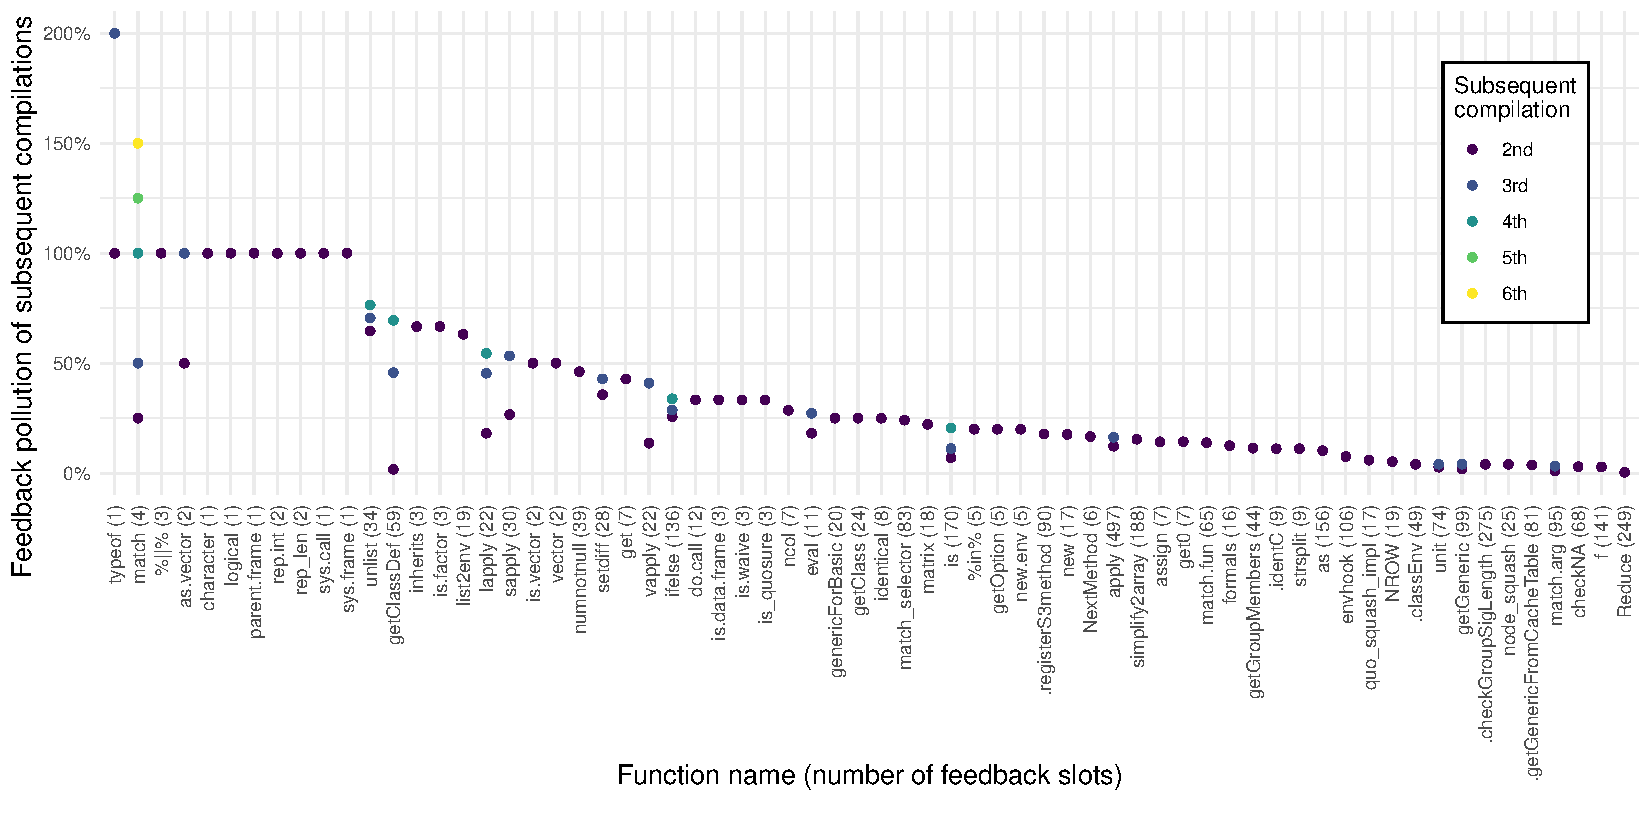
\includegraphics[width=1.3\textwidth]{figures/pollution/master/kaggle-function-pollution.pdf}
	\end{adjustwidth}
	\caption{Function pollution in Kaggle script, each point represents a compilation\cite{feedback-vmil}}\label{fig:kaggle-pollution}
\end{figure}

When we take as an example the function \texttt{typeof}, we have three compilations. The second compilation has a 100\% polluting and the third a 200\% pollution, meaning that both of the recompilations use all slots as polluted. The function is a wrapper around a C function that returns the type of the argument. It has a single parameter, to which the slot is connected to, and since it can be called with any type, it will always pollute when a new type is observed.

Looking at the benchmarks, we have observed much less compilations than in the Kaggle code. This is to be expected, as the benchmarks are mostly small numerical programs. In figure \ref{fig:bench-pollution} we can see the \textit{benchmark pollution}, which is the ratio of polluted recompilations out of all recompilations. Out of the 16 selected benchmarks, 10 of them have at least one polluted compilation. The overall ratio between polluted compilations is 8.2\%, which is very similar to the 10.9\% observed in the Kaggle code, but when looking at the function pollution, we have observed that out of 139 compiled functions there are 21 polluted functions (15.1\%). This is very likely due to the nature of the benchmarks, as they are numeric programs which are mostly using very few types. Still, a pollution can be observed and should be prevented.

\begin{figure}
	\centering
	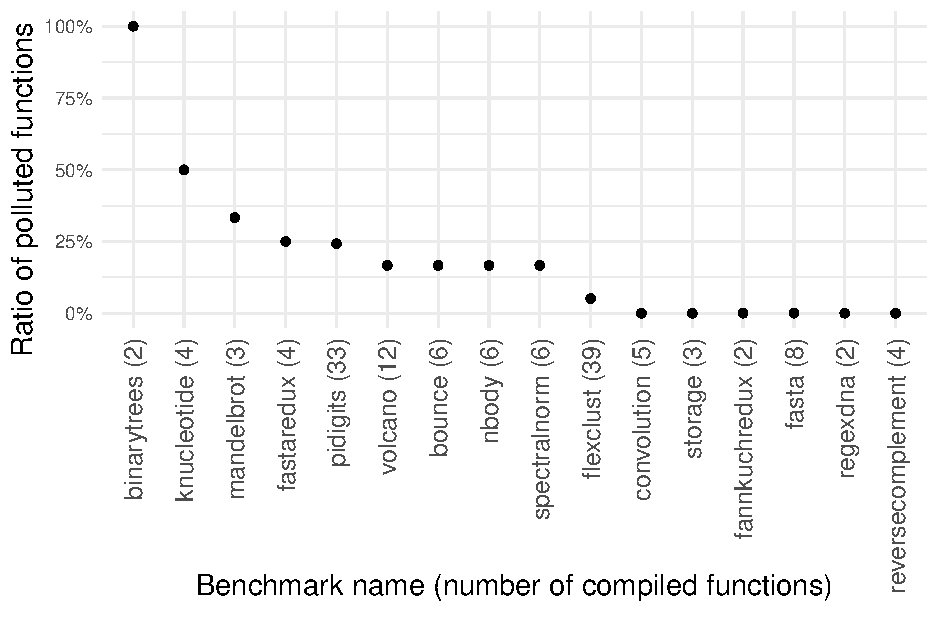
\includegraphics[width=0.7\textwidth]{figures/pollution/master/benchmark-pollutionBW.pdf}
	\caption{Pollution of functions in benchmarks\cite{feedback-vmil}}\label{fig:bench-pollution}
\end{figure}

Splitting the pollution by a feedback slot type, the observed values are taking most of the pollution. Out of the 11,199 slots in the Kaggle code, 0.5\% of observed calls, 2.7\% of observed tests, and 5.7\% of observed values are polluted. This is not surprising, as the type feedback slots are the slots with most variability.

\todo{the polymorphic functions}

%---------------------------------------------------------------
\subsubsection*{Summary}
%---------------------------------------------------------------

In table \ref{tbl:pollution-summary} is a summary of the feedback compilation in the benchmarks and in the Kaggle code. We can see that feedback pollution happens in both the Kaggle code as well as in the benchmarks, although the benchmarks have a lower pollution rates, mostl likely due to the stable nature of the code.

We have observed that pollution is most likely caused by polymorphic functions that are called often with different types, but other causes for pollution can be a global state.

Most of the polluted slots are the observed values.

\begin{table}[H]
	\centering
	\begin{tabular}{llll}
		\hline
		                      & Kaggle      & Benchmarks  \\
		\hline
		Lines of code         & 108         & 1268        \\
		Compilations          & 970         & 257         \\
		Polluted compilations & 90 (10.9\%) & 21 (8.2\%)  \\
		Compiled functions    & 315         & 139         \\
		Polluted functions    & 66 (21\%)   & 21 (15.1\%) \\
		\hline
	\end{tabular}
  \caption{Summary of the feedback pollution in the corpus\cite{feedback-vmil}}\label{tbl:pollution-summary}
\end{table}


The code of the analysis is freely available at GitLab\footnote{\url{https://gitlab.com/rirvm/splitfeedback-experiments/-/tree/artifact}} as part of the VMIL paper\cite{feedback-vmil} aritfact.

%---------------------------------------------------------------
\section{Pollution prevention}
%---------------------------------------------------------------

After observing that a feedback pollution is a real phenomenon, we propose a way to reduce it.

One way to reduce the pollution is to split the feedback vector into multiple different ones. Since Ř already employs a contextual dispatch, the constructed dispatch could be reused by the feedback, constructing a unique vector for each call context the function is invoked with. A split feedback was implemented by Michal Štěpánek as a part of his master thesis\cite{michal2025obohaceny}. However, this solution brought new problems, as now the observed information is much sparser and needs to be merged from multiple vectors. Splitting the feedback also negativaly impacts the interpreter performance, and complicates function compilation.

Another approach would be to implement a \textit{feedback decay}. The idea is that the feedback information in every slot would slowly \textit{decay} as new information is observed. This will need to be finely tuned, as very quickly the JIT could be stuck in a \textit{deopt loop}, compiling a function just to trigger a deoptimization next time it is invoked.

%---------------------------------------------------------------
\chapter{Feedback Usage}
%---------------------------------------------------------------

\begin{chapterabstract}
	After observing that the feedback vector can be polluted with information, the next step is the understanding of how the feedback is used in the compilation. Ultimately, we want to categorize slots in how they are used, and quantify how much of the recorded information influences the compilation, as well as identifying the reason for why slot was not used in a compilation. First, we define the categories of how a slot can be used or not used. Next we analyze the usage of feedback in Ř. Lastly, we acknowledge the limitations of the analysis and discus alternative approaches.
\end{chapterabstract}

In this chapter, we only focus on the \textit{type slots} because, as observed in the feedback pollution analysis, these suffer from pollution the most. They are also the most variable parts, and having a much larger state space they allow for a richer analysis.

%---------------------------------------------------------------
\section{Definitions}
%---------------------------------------------------------------

First, we define an \textit{non-empty slot} as a slot that has at least one observation. An empty slot means that the observed instruction was never executed, thus it is part of a program which is not executed.

We say that a slot is \textit{referenced} if it is part of a function that is compiled to native, including slots inside of inlined functions. A slot is then \textit{read} if during this compilation the information in the slot is observed. A \textit{used slot} is a type feedback slot that has an assumption connected with it in the final version of PIR (after all optimizations finished running). A used slot is always non-empty as we cannot assume a type if we have not observed any.

%---------------------------------------------------------------
\subsubsection*{Used Slots}
%---------------------------------------------------------------

When an assumption on a type is emited, it has a structure outlined in listing \ref{lst:assume-structure}. The value we speculate on is in the register \texttt{\%1} with a \textit{static type}, which is inferred from the call context, known types of builtins, and preceding assumptions. The instruction has also an associated \textit{feedback type}, which is the union of types observed in the interpreter. The speculated value is an input to an \texttt{IsType} instruction, which checks the actual runtime type against the \textit{assumed type}. The result of the type check is then an input to the \texttt{Assume} instruction, along with the corresponding \texttt{Checkpoint}. If the type check fails (\texttt{\%2} is false), we trigger a deoptimization and restore the frame state according to the checkpoint, otherwise we continue with the execution.

\begin{listing}[H]
	\centering
	\begin{minted}[linenos=false]{\pirlexer}
<static type>   %1    = <instruction>       args... <feedback type>
lgl$#-          %2    = IsType              %1 isA <assumed type>
void                    Assume              %2, <checkpoint> (Typecheck[Type#N])
  \end{minted}
	\caption{PIR code structure of type assumption}\label{lst:assume-structure}
\end{listing}

The construction of the assumed type is not as straight-forward as it might seem (illustrated in figure \ref{fig:types-venn}). First, we construct an \textit{expected type} by intersecting the static and feedback type. If this intersection is empty, no assumption is emited and the feedback type is empty, otherwise we procede to create the assumed type.

\begin{figure}
	\centering
	\includediagram{8}
	\caption{Illustration of the relationship between static, feedback, expected and assumed types}\label{fig:types-venn}
\end{figure}

It can happen that the static type is more precise than the feedback type, and the feedback type is not a subtype of the expected type (in the figure \ref{fig:types-venn}, the green area is non-empty). We call this a \textit{narrowing} of the feedback type with the static type. For example, this happens when we statically know that the value we are speculating on is a scalar, but we have observed also non-scalar values.

If the R type of the expected type is not integer, float or logical vector, we do not speculate on it as it is. The optimizations are not able to use this precise of an information, thus the compiler tries to relax the assumption first. We call this \textit{widening}, as we are widening the information of the feedback type (and also the expected type), while still staying in the bounds of the static type. This results in the final assumed type. If we cannot reasonably relax the type, we give up on assuming.

If the assumed type is equal to the feedback type, we say that the feedback was used as \textit{exact match}. This implies that it has not been narrowed, nor widened.

%---------------------------------------------------------------
\subsubsection*{Unused Slots}
%---------------------------------------------------------------

\todo{throw away the example?}

For the unused slots, we want to understand what is the reason why they are not used. For illustration, we are going to use the example in listing \ref{lst:unused-example}. When we look at the RIR code generated after at least one execution of the function \texttt{f}, we see that there are six type feedback slots. Four of them have recorded the type of integer scalar, corresponding to the two loads of global variable \texttt{G} and their addition, one slot has observed the type double as a result of the second addition and coercion of integer to double, and one slot is empty due to being in an unreachable branch. The final PIR code has a single assumption on the type of the global variable \texttt{G}.

In the final PIR in listing \ref{lst:unused-example-pir}, we only see three instruction with attached type feedback (lines 5, 11 and 13), corresponding to the feedback slots 0, 2 and 5. We say that the other slots are \textit{optimized away}. In our example, the instruction connected with slot 3 is removed because it is in unreachable branch, whereas the slots 1 and 4 are optimized away because the loading of variables is optimized to only use registers.

Another reason for not using a slot is because it contains \textit{redundant information}. The slots 0, 1, 2 and 4 contain exactly the same information, because they all depend on the type of \texttt{G}. Since we assume on the slot 0, it is used, but we do not need to create any further assumptions, as the type is know statically. Formally we say that an \textit{unused slot is redundant} if its type information is equivalent to any other slot, both used or unused. Note that reduntant slots and slots that are optimized away are not disjunct categories.

\begin{listing}[p]
	\begin{minipage}{0.47\textwidth}
		\begin{minted}{R}
G <- 42L
H <- 42

f <- function() {
    x <- G + G
    if (FALSE) {
        return(H)
    }
    x + 42
}
    \end{minted}
		\subcaption{R code}
	\end{minipage}
	\hfill
	\begin{minipage}{0.47\textwidth}
		\begin{minted}{\rirlexer}
0:
      0   ldvar_cached_  G{1}
      9   [ integer (s) | value ] Type#0
     14   ldvar_cached_  G{1}
     23   [ integer (s) | value ] Type#1
     28   ; +(G, G)
          add_
     29   [ integer (s) ] Type#2
     34   stvar_cached_  x{0}
     43   push_  FALSE
     48   visible_
     49   asbool_
     50   brtrue_  1
     55   br_  2
1:
     60   ldvar_cached_  H{2}
     69   [ <?> ] Type#3
     74   ret_
2:
     75   ldvar_cached_  x{0}
     84   [ integer (s) | value ] Type#4
     89   push_  42
     94   visible_
     95   ; +(x, 42)
          add_
     96   [ double (s) ] Type#5
    101   ret_
    \end{minted}
		\subcaption{RIR code of function \texttt{f}}
	\end{minipage}
	\vfill
	\begin{adjustwidth}{-1cm}{-1cm}
		\begin{minipage}{\textwidth}
			\begin{minted}{\pirlexer}
BB0
  goto BB1
BB1   <- [0]
  val?^ | miss    %1.0  = LdVar              G, R_GlobalEnv
  val?            %1.1  = Force!<value>      %1.0,    <int$->
  lgl$#-          %1.2  = IsType             %1.1 isA int$-
  cp              %1.3  = Checkpoint          -> BB2 (default) | BB3 (if assume failed)
BB2   <- [1]
  void                    Assume             %1.2, %1.3 (Typecheck[Type#0])
  int$-           %2.1  = CastType           dn %1.1
  int$-           %2.2  = Add                %2.1, %2.1, elided   <int$->
  void                    Visible
  real$-          %2.4  = Add                %2.2, 42, elided   <real$->
  void                    Return             %2.4
      \end{minted}
			\subcaption{Optimized PIR code of the function \texttt{f}}\label{lst:unused-example-pir}
		\end{minipage}
		\caption{Example of type slots categories}\label{lst:unused-example}
	\end{adjustwidth}
\end{listing}

Because we can infer that the type of the return value from the surrounding context, we might want to also detect that the last slot is dependent, even though it has a different type. However this proved to be very difficult. Due to how types in Ř are compiled, we are unable to track the origin of a type information, and thus we can only track simple dependencies. On the other hand, this definition of redundant slots might be too general in certain cases where slots have same type from different reasons, but again, we are unable to track that. \todo{move to limitations?}

There are more reasons to why a slot might not be used, like the information in the feedback not being useful for speculation, the information being overriden by static information, or that the slot is too polluted. We do not categorize these further, as they do not play with slot pollution significantlly \todo{rewrite}.

%---------------------------------------------------------------
\subsubsection*{Polymorphic Slots}
%---------------------------------------------------------------

A \textit{polymorphic slot} is slot that has observed more than one distinct type. This is a superset of the \textit{polluted slots}, because if a slot is polluted, it has to have two different non-empty values between the compilation, thus there had to be at least two recordings of different type. A non-polymorphic slot is \textit{monomorphic}.

Observing polymorphic slots allows us to outline the usage of polluted slots, while also observing the behaviour of slots that have (potentially) too general of an information even before the first compilation.

%---------------------------------------------------------------
\section{Methodology}
%---------------------------------------------------------------

In order to collect all the information needed, we had to directly instrument the Ř compiler. We inspect the PIR code of closures and collect information about all of the assumptions, including the corresponding type test and cast instructions. We use the rich Ř APIs for traversing code and inspecting instructions. All of the analysis code is in the main repository in the branch \texttt{feedback-in-jits}\footnote{\url{https://github.com/reactorlabs/rir/tree/0137c1ad4ddbcc8e035e86a317e5dbe6b645deb6}}.

Our unit for collecting information is a \textit{closure version compilation}. This is one lowering of a closure from PIR to native code. For each compilation, we define its \textit{universe} as the compiled closure and all of its inlinees. All counts are then in reference to this universe, so for example the number of referenced slot of one compilation is the sum of all slots in the universe. We ignore multiple inlinings of the same closure in one compilation as we have observed that in most cases the slots are used in the same way across all inlinings.

The final data is aggregated over these closure version compilations. Thus when we say that there were two used slots, we mean that over all compilations, a slot was used two times, it might even be the same slot. The reason for this was that between the individual compilations, the state of the slots can change, and there is no reasonable way to reference and quantify all slots after the program terminates.

\begin{table}[ht]
	\makebox[\linewidth]{%
		\begin{tabular}{l l l l l}
			\hline
			\textbf{Program name}   & \textbf{Benchmark suite} & \textbf{Lines of code} & \textbf{Compilations} & \textbf{Referenced slots} \\
			\hline
			bounce\_nonames\_simple & Are We Fast Yet          & 58                     & 11                    & 264                       \\
			mandelbrot              & Are We Fast Yet          & 65                     & 14                    & 358                       \\
			flexclust\_no\_s4       & Real Thing               & 163                    & 144                   & 5335                      \\
			volcano                 & Real Thing               & 63                     & 23                    & 2037                      \\
			binarytrees\_naive      & Shootout                 & 31                     & 22                    & 1070                      \\
			fannkuchredux           & Shootout                 & 63                     & 6                     & 251                       \\
			fannkuchredux\_naive    & Shootout                 & 62                     & 5                     & 244                       \\
			fasta\_naive\_2         & Shootout                 & 88                     & 17                    & 598                       \\
			knucleotide             & Shootout                 & 72                     & 59                    & 1493                      \\
			pidigits/pidigits       & Shootout                 & 333                    & 92                    & 5651                      \\
			titanic                 & -                        & 108                    & 2020                  & 66119                     \\
			\hline
		\end{tabular}
	}
	\caption{Overview of analyzed programs}\label{tbl:analysis-overview}
\end{table}

We run the analysis on a selection of ten benchmarks from the benchmark suite and the Titanic Kaggle notebook, outlined in table \ref{tbl:analysis-overview}. We can see that the Kaggle notebook has more compilations by an order of magnitude when compared to the benchmarks and thus also many more referenced slots. All of the experiments were ran with OSR compilations turned off and with the the invocation threshold for native compilation set to 10 \todo{justify}.

%---------------------------------------------------------------
\section{Observations}
%---------------------------------------------------------------

\todo{figures labels, adjust them so they do not overflow}

In constrast to the pollution analysis, while categorizing the slots we have observed that the Kaggle script behaves very much in the same way as the benchmark programs do. This is interesting, because they are written in very different ways and are doing different computations. It might point to a deeper issue, either connected with the behavior the Ř compiler.

In figure \ref{fig:graph-overview} is the categorization of used slots. We can see that most of the slots are not empty (68\% on average) and most of the non-empty slots are read (81\% on average), thus are considered for speculation. But on average only 14\% of slots are used, (21\% of non-empty slots). This is surprising, as the recording of information is impacting the speed the bytecode interpreter, and yet the recorded information is used quite sparsely.

A hypothesis we had was that a polymorphic slot is less likely to be used. Out of the polymorphic slots, 25\% of them are used, compared to the non-empty monomorphic slots where 21\% are used. This might lead to a conclusion that by a slot being polymorphic it is more likely to be used. However it is probably due to the fact that by their nature, polymorphic slots are on the paths of the program which are executed, thus there are less reasons to not use them.

\begin{figure}
	\centering
	\begin{adjustwidth}{-3cm}{-3cm}
		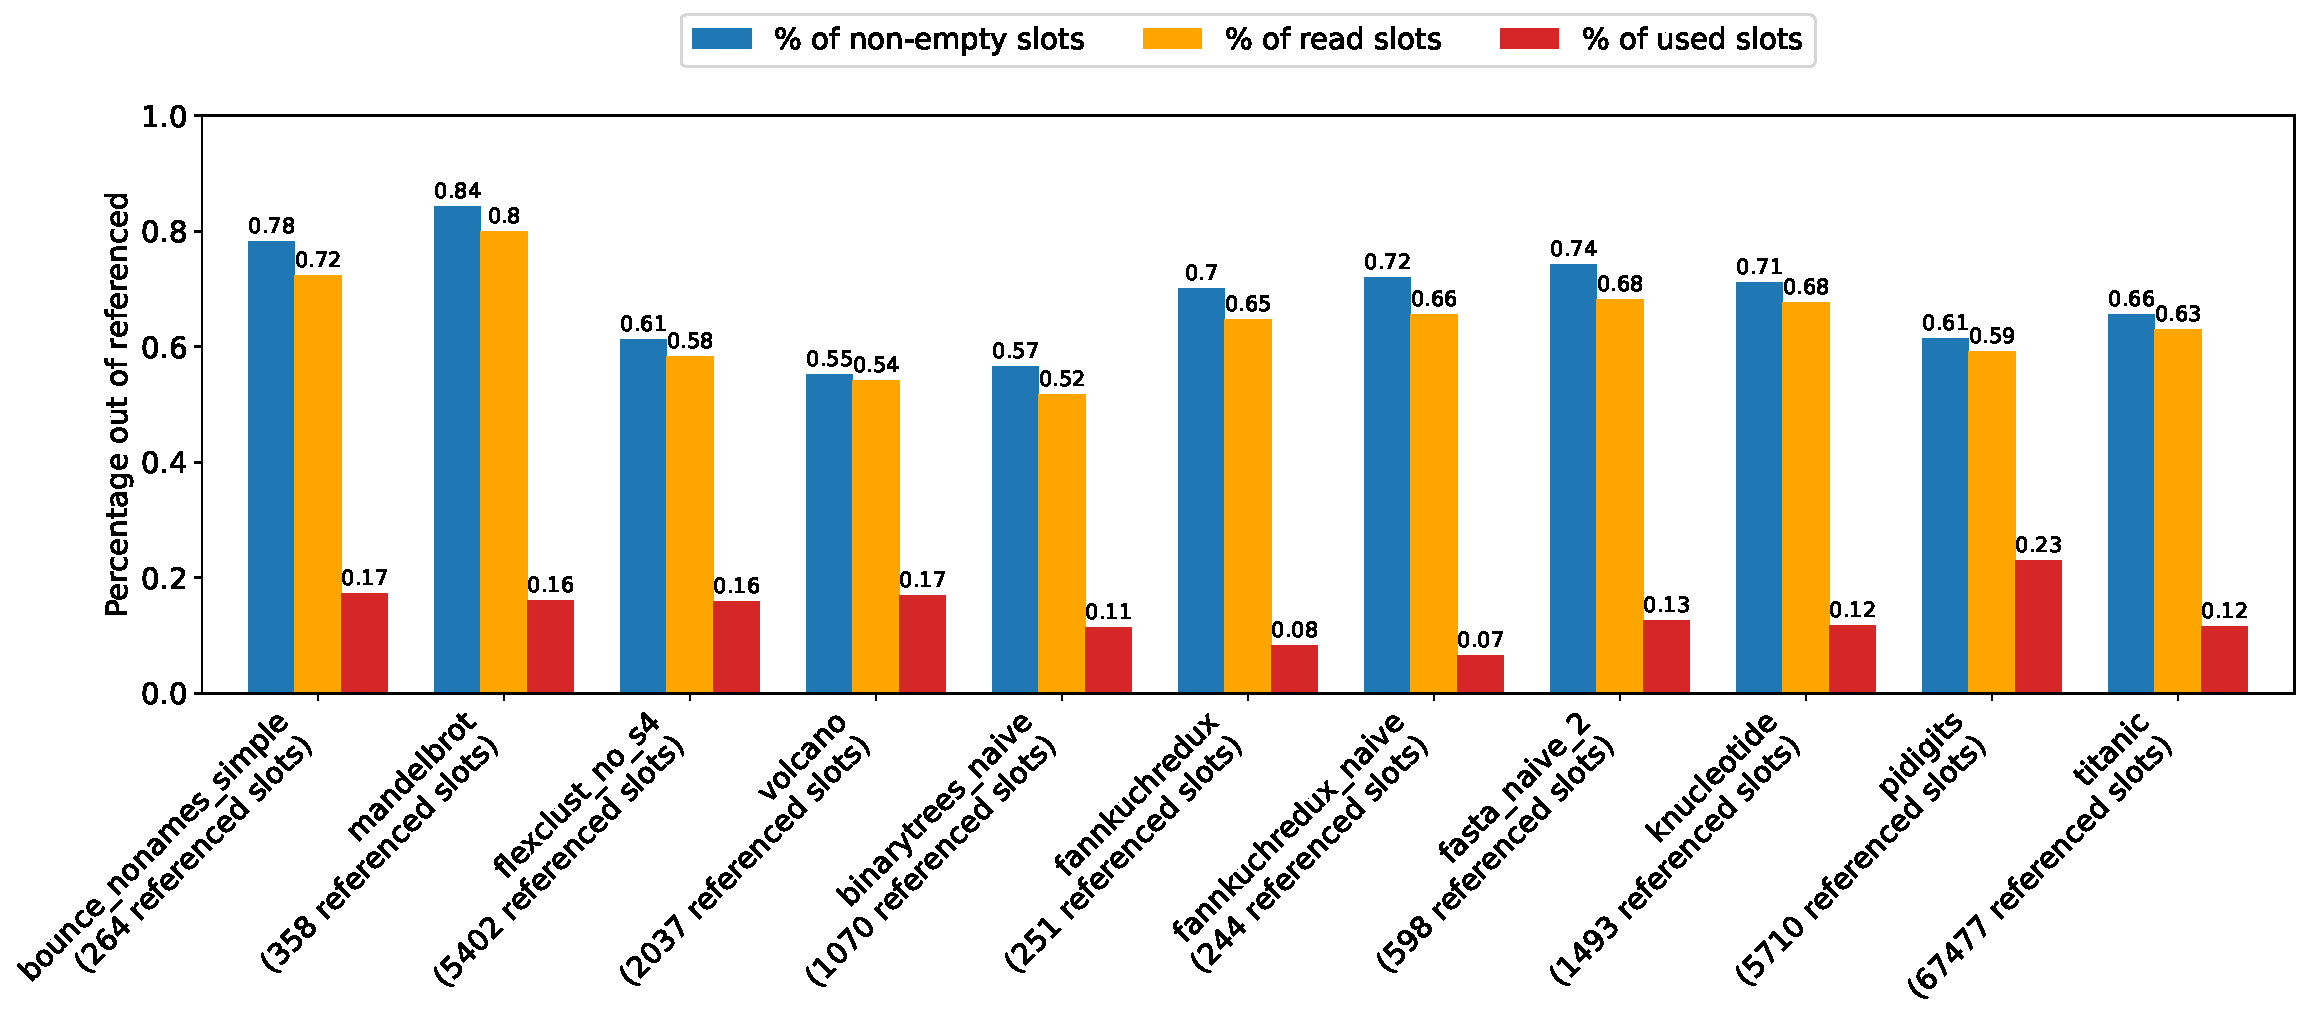
\includegraphics[width=1.5\textwidth]{figures/usage_overall.pdf}
	\end{adjustwidth}
	\caption{Usage of slots across closure compilations}\label{fig:graph-overview}
\end{figure}

When we consider the unused slots shown in figure \ref{fig:graph-unused}, we can see that the dominating cause for a slot not being used is redundancy, on average 59\%. This is expected in the benchmarks because they usually only use one numeric type across the whole program. But the Kaggle script uses a lot of different types, yet 58\% of the unused slots are deemed redundant, which is lower than the average. This leads us to believe that there is a deeper cause for a redundant slot, either in the behavior of R, or in the way the information is observed in the interpreter.

\todo{optimized away}

25\% of all slots are neither redundant nor optimized away. This might include some actually redundant slots that are not caught by our approximate analysis, but there might also be other reasons for not using a slot, such as the information in it being too general, and these will probably overlap with the identified reasons. These need to be further analyzed.

\begin{figure}
	\centering
	\begin{adjustwidth}{-3cm}{-3cm}
		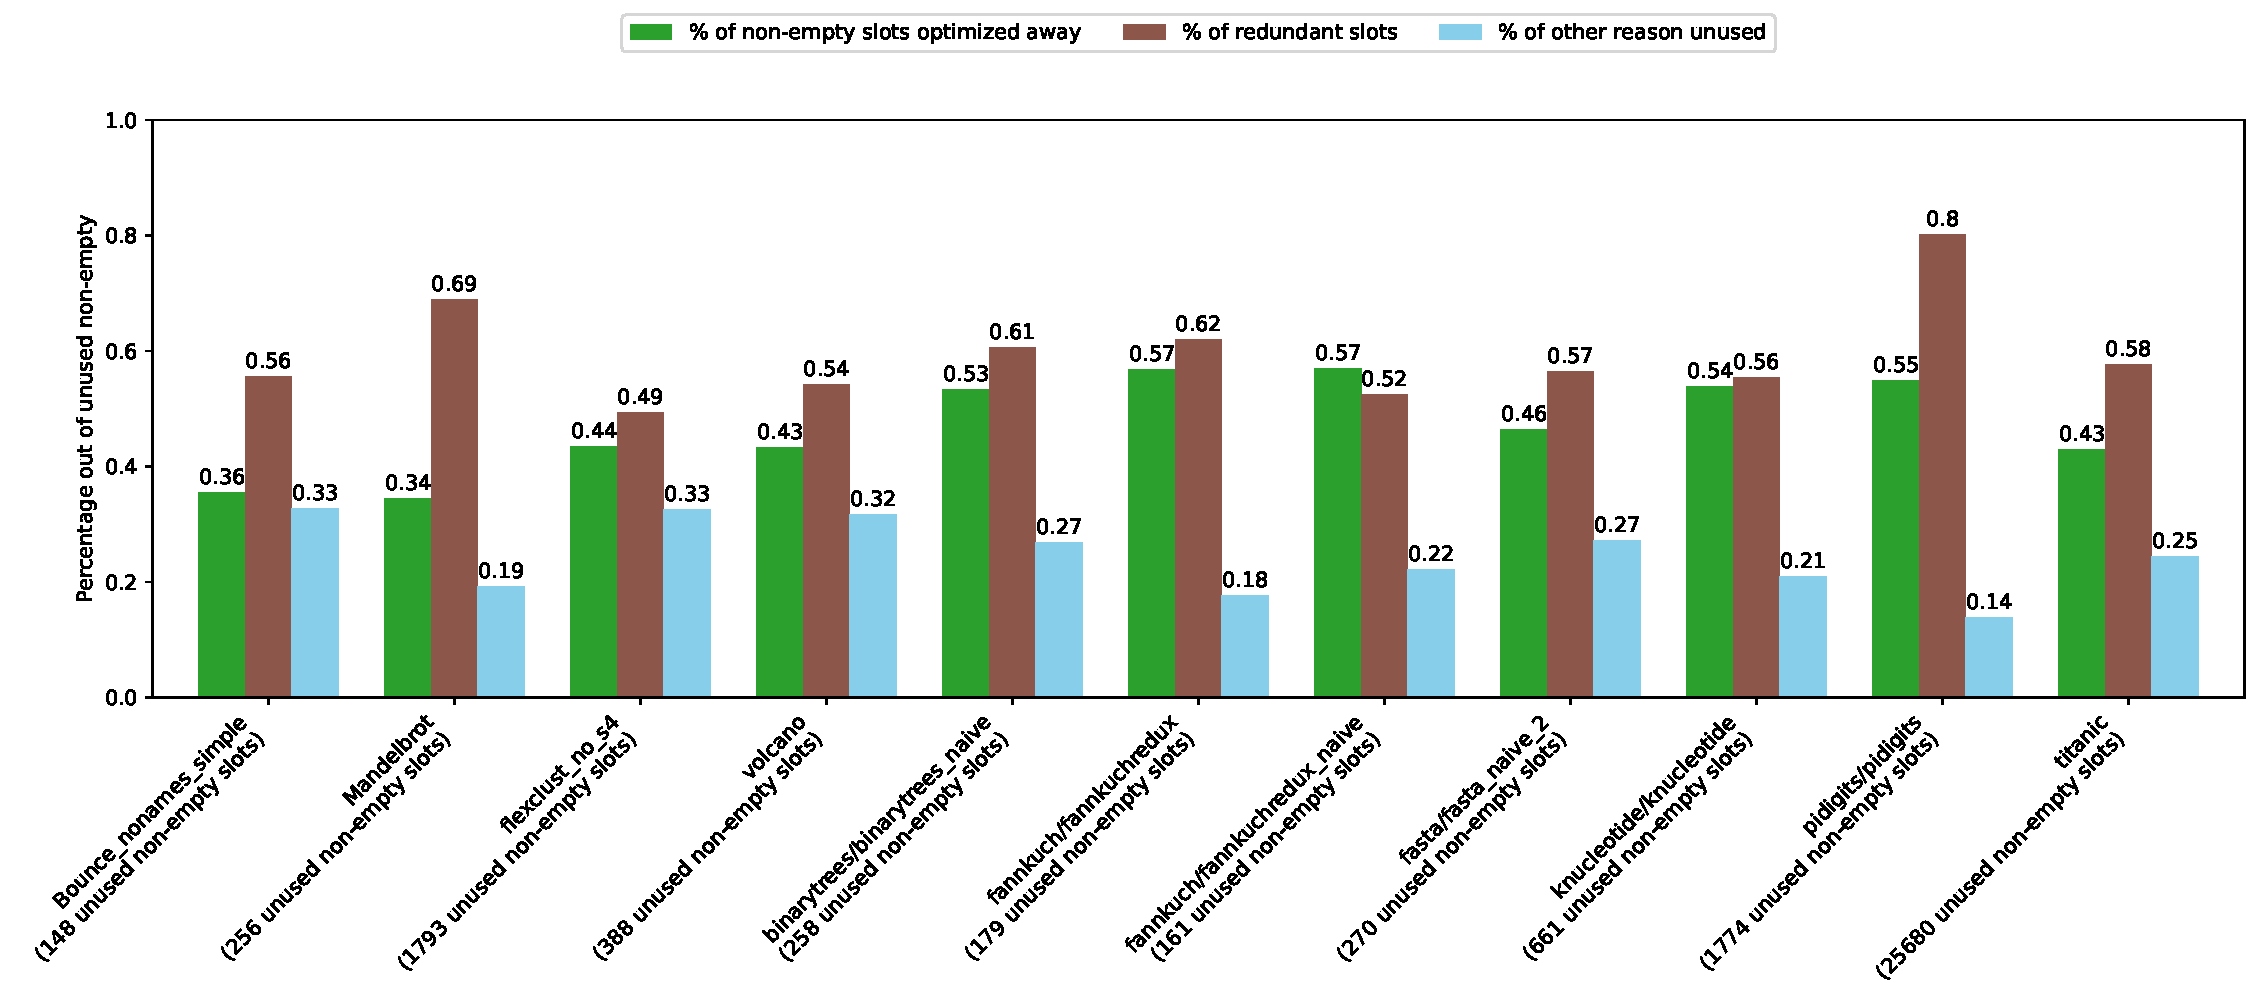
\includegraphics[width=1.5\textwidth]{figures/unused.pdf}
	\end{adjustwidth}
	\caption{Categorization of unused slots across closure compilations}\label{fig:graph-unused}
\end{figure}

\todo{exact numbers, not averages}
When we look on the graph \ref{fig:graph-used}, we can see that more than half of the slots are used as exact match. If we split the monomorphic and polymorphic used slots, we can see an even bigger distinction. On average 81\% of used monomorphic slots are used as exact match. This means that most of the time, when a slot is not polymorphic, it contains an information precise enough to be used as it is. On the other hand, 93\% of used polymorphic slots are widened. This is to be expected, as the polymorphic slots have usually a more general type that does not pass the check for a slot to be used as it is.

For the polymorphic slots used as exact match, the feedback type is either a single non-scalar R type (integer, real or logical), or any R type which might be missing. In either case, the type is always not scalar and we have observed that it is not an object or even that it does not have any attributes. The polymorphism in these cases probably come from observing both scalar and non-scalar types.

Interestingly, there are very few slots that are narrowed by the static information, 18 to be precise.

\begin{itemize}
	\item{} 2 of them have added information about the type not being NA. Since we do not record this information\footnote{In order to observe that a vector is not NA, we would need to inspect all elements of it and this is very costly for large vectors}, it is trivial for the static type to narrow it in this way. These are the only monomorphic slots that are narrowed.
	\item{} 4 slots are narrowed into a scalar type. This is due to the slot observing also non-scalar types, but the static type can specialize the observation.
	\item{} 2 slots have their type narrowed to a double and the only information used from the slot is that the value does not have attributes.
	\item{} In 9 cases, the static type removes a \enquote{might be missing} attribute from the feedback type. In these cases we have observed too many values and the type feedback falls back to the most generic type, which has the attribute that it might be a missing value. But this speculation is on a \texttt{Force} instruction, which when forcing a value that is missing result in an error, thus the result of \texttt{Force} is always not missing or it diverges.
\end{itemize}

\todo{For the used slots - only show the avergaes per all/monomorphic/polymorphic?}

\begin{figure}[t]
	\centering
	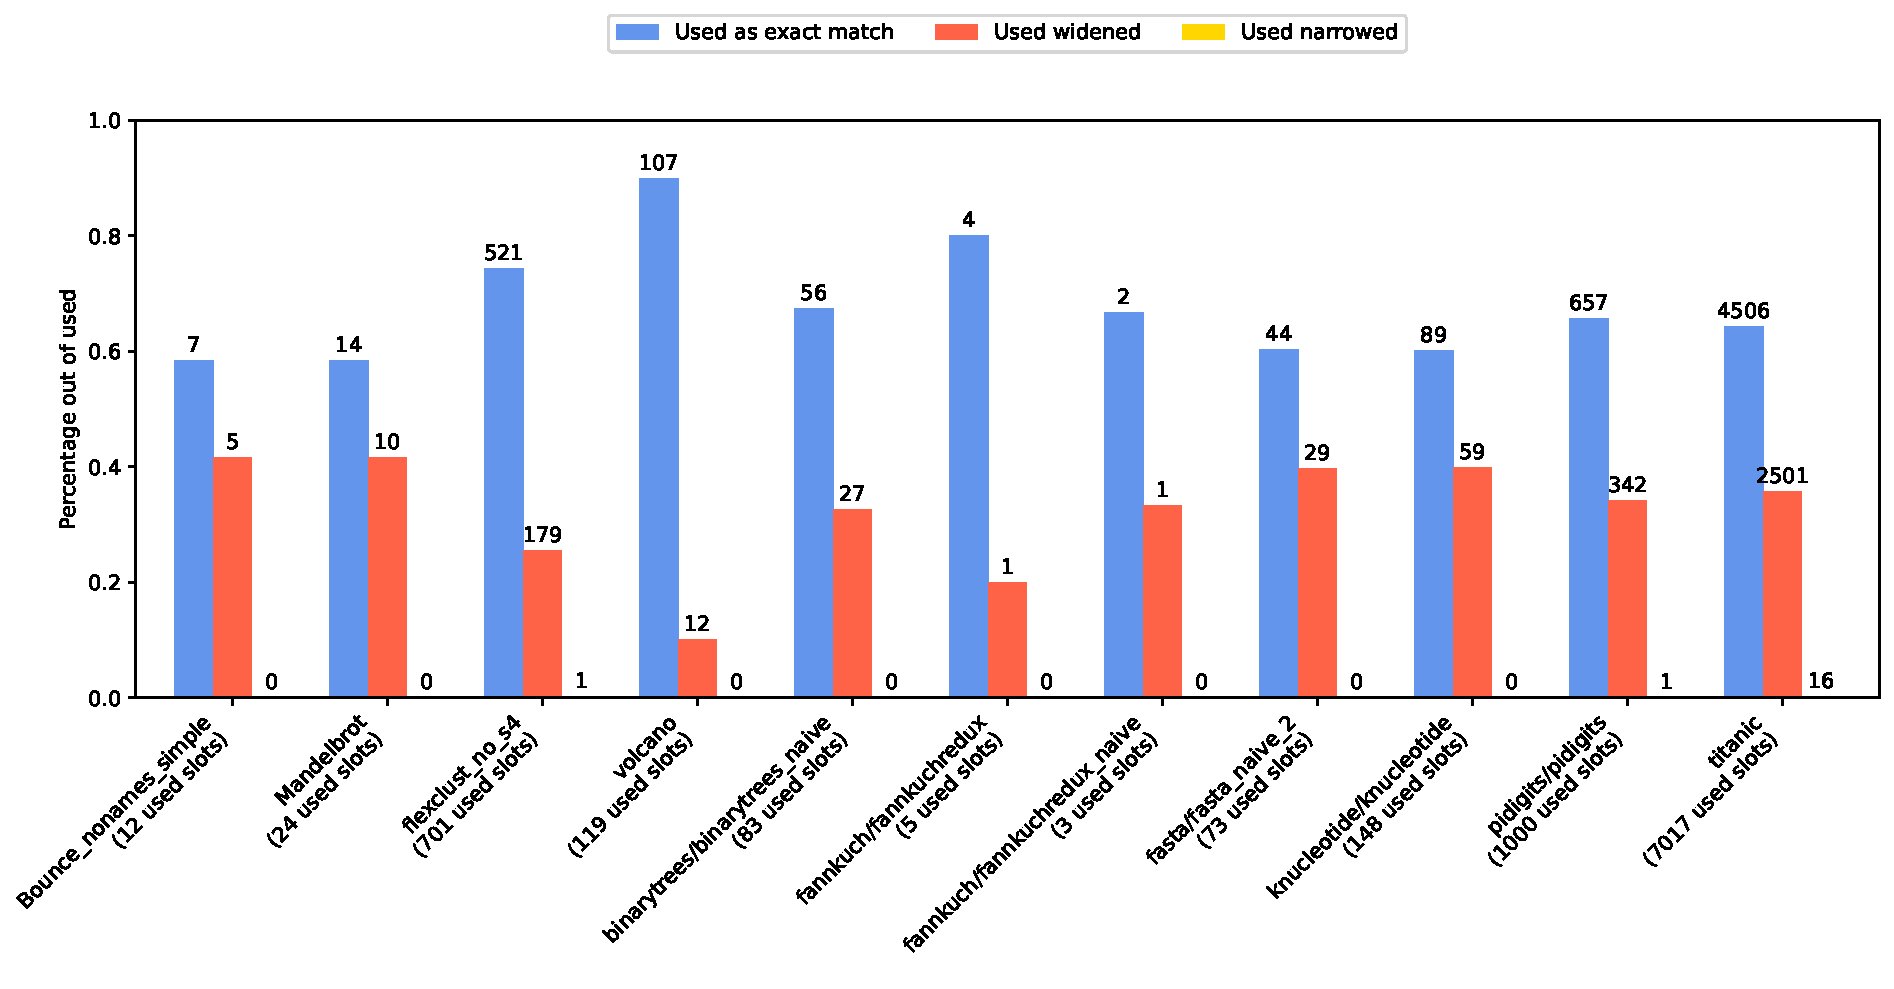
\includegraphics[width=0.7\textwidth]{figures/used.pdf}
	\caption{Categorization of used slots}\label{fig:graph-used}
\end{figure}

\begin{figure}[t]
	\centering
	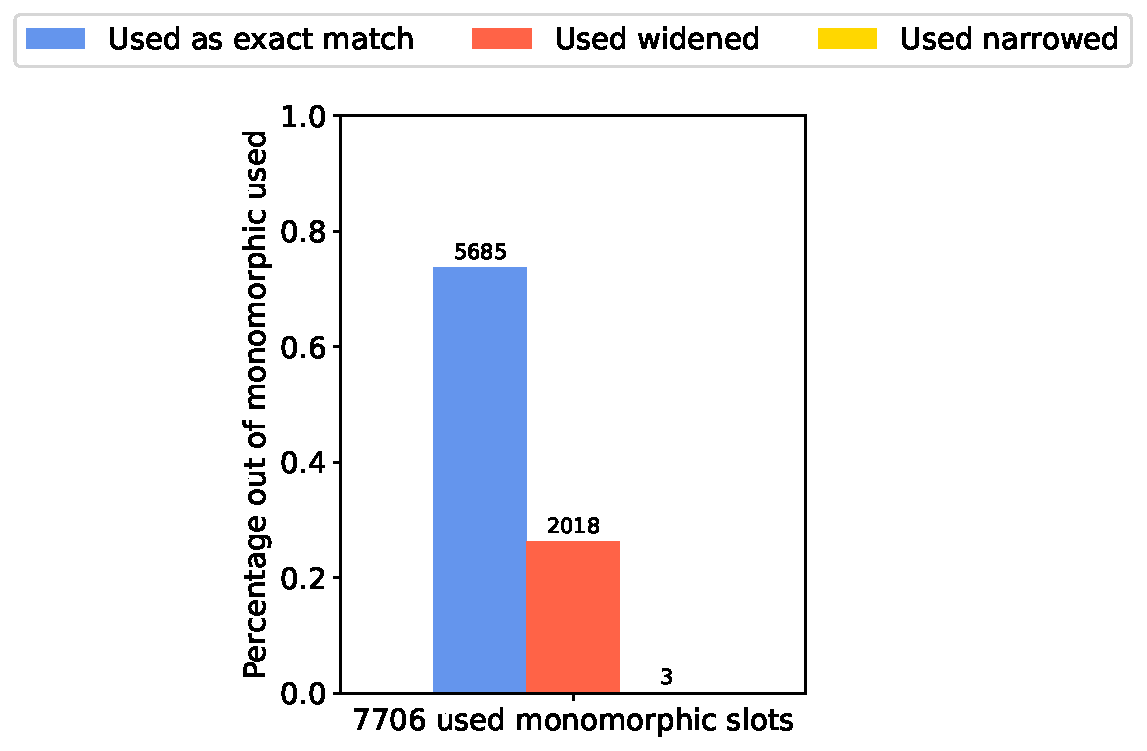
\includegraphics[width=0.7\textwidth]{figures/used_monomorphic.pdf}
	\caption{Categorization of monomorphic used slots}\label{fig:graph-used-mono}
\end{figure}

\begin{figure}[t]
	\centering
	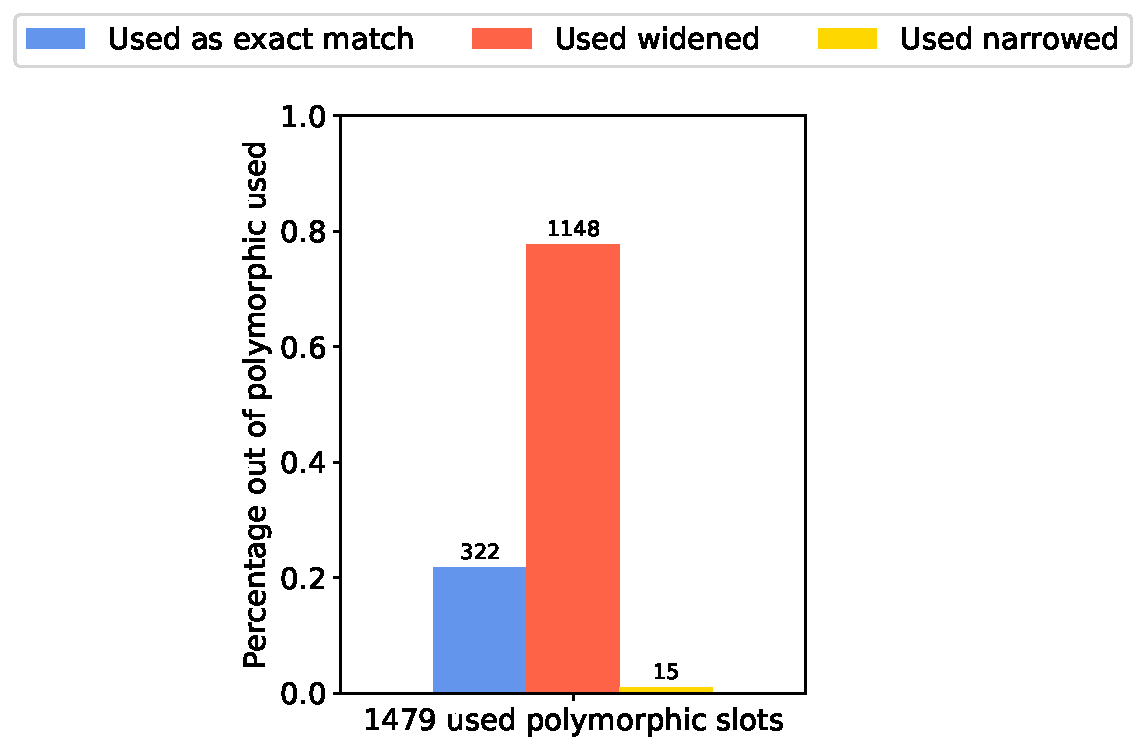
\includegraphics[width=0.7\textwidth]{figures/used_polymorphic.pdf}
	\caption{Categorization of polymorphic used slots}\label{fig:graph-used-poly}
\end{figure}

%---------------------------------------------------------------
\subsubsection*{Conclusion}
%---------------------------------------------------------------

The main takeaway of the analysis is that a very low number of feedback slots is being used by the compiler. This leads to a time spent in the interpreter by recording observations being wasted. If we are able to detect which slots are truly redundant, we could optimize

Another key point is that a polymorphism, and by extend pollution, does not impact \textit{if} a slot is used in compilation, but it influences \textit{how} the feedback is used. Thus by reducing the feedback pollution we would not be significantly influencing if a slot is used, but we might improve the available optimizations by having more precise information.

\todo{bit more}

%---------------------------------------------------------------
\section{Limitations}
%---------------------------------------------------------------

The biggest drawback of the analysis is the analysis of inlined functions. It is not uncommon that a funciton is inlined more than once in a single closure compilation, and this proves to be difficult, as one slot might be used differently or used in one case and not used in the other. At the same time, inlining a function many times is going to skew the numbers of the used slots. In our experiments, we have observed very few slots that were used differently in multiple places, thus we chose to ignore these duplications.

\todo{redundant section; merge with the stuff in motivation}
The definition of a redundant slot is very broad and might catch some slots that are not dependent, while at the same time not catch slots that are dependent, but capture a different type. Lets take an example function \texttt{function(x) x + 42}. This function has two type slots, one for the loading of argument \texttt{x} and the second is for the result of \texttt{+}. If we call this funciton with an integer, we record two different types, integer scalar in the first and a double scalar in the second (integer gets coerced into a double). Our analysis will not report any dependency, but from the argument types we truly know the result type. This would require a much more advanced instrumentation of the compiler and might be even

The analysis of usage is also quite broad, but due to the architecture of Ř we are unable to observe nor reconstruct how a paricular type of an instruction is constructed. Ideally we would like to be able to say precisely which parts of the feedback are used and in which instrucitons, but this would probably lead to a whole refactoring of the compiler.

\todo{unstable benchmarks and titanic}

%---------------------------------------------------------------
\chapter{Related Work}
%---------------------------------------------------------------

%---------------------------------------------------------------
\chapter*{Conclusion}\addcontentsline{toc}{chapter}{Conclusion}\markboth{Conclusion}{Conclusion}
%---------------------------------------------------------------

The main goal of this thesis was to implement a tool which would help us to look under the lid of the JIT compiler pot, to increase its observability. Such tool should then allow us to study a different phenomenons that happen along the dynamic compilations the JIT performs. Concretely, we were motivated to understand the behavior of the feedback the compiler uses for generating code.

We implemented this tool as described in chapter 2, and as of now it is part of the Ř compiler codebase. We were able to minimize the impact on the rest of the compiler to a minimum by using conditional compilation and a series of hooks, simple functions that capture the state of the compiler at various points of execution and compilation.

Based on this tool, we were able to perform an analysis of the feedback pollution in Ř, as outlined in the chapter 3 and VMIL paper\cite{feedback-vmil}. We observed that feedback pollution happens in approximately 19\% of compilations. We also present ways we could implement a reduction of the pollution, either by splitting the feedback vector by context, or by introducing a feedback decay.

Continuing the observations about the feedback vector, we evaluated how the recorded type information is used during compilation. We observed that a very small number of recorded information is used (21\% of feedback vector slots on average). We also conclude that if a feedback vector slot is polymorphic, and by extend a polluted, it does not affect if it is going to be used, but it weakens the speculations that the compiler can assume on. Furhtermore, we identified different reasons why a feedback information is not used, namely that it contains duplicite information, or the instruction we record the feedback for is optimized away.

%---------------------------------------------------------------
\section*{Future Work}
%---------------------------------------------------------------

The main question we are currently unable to answer is \textit{how much the feedback pollution and low usage of feedback information impact the performance of real programs}. This is a very hard question to answer, as at this point we do not have the information about performance impacts of the various components. We are unsure of about how much time is spent in the interpreter, recording feedback information, in the JIT compiled code, in the builtin functions of GNU-R, or in the native extensions of libraries. Based on these metrics, we would be able to assess the real-world impact of the observations and priorotize optimizations for the most affected parts of the compiler.

Nonetheless, the observations made as a part of this thesis unlock for us multiple ways we could advance the JIT compiler.

%---------------------------------------------------------------
\subsubsection*{Reducing Pollution}
%---------------------------------------------------------------

In order to properly analyze how a polluted slot affects the runtime performance of JIT compiled code, we would need an \textit{oracle} that at a point of compilation would be able to correctly return an \textit{ideal feedback vector} such that the compilation produces as optimized code as possible. Since we want to observe the behavior of real-world programs, it is unfeasable to hand-write this oracle for every compilation.

We could achieve at least an approximate oracle by extending the recording tool by its counterpart that would be able to \textit{replay} the recorded information, i.e. infulence a compilation based on previous observations. Iteratively, we would run the program with the trace of the previous run as an additional input from which it would approximate the ideal feedback vector.

%---------------------------------------------------------------
\subsubsection*{Reducing Recoding}
%---------------------------------------------------------------

Another angle to take is reducing the time spent recording the feedback information in the interpreter.

If we are able to statically find redundant feedback slots and therefore eliminate some number of recording instructions, we should be able to speed up the interpreter, but this should not be to the detrement of JIT compilation. Another angle would be to dynamically observe which slots are being used and which are not and based on this trace conditionaly turn off recording of certain slots.

%---------------------------------------------------------------
\subsubsection*{Relaxing Assumptions}
%---------------------------------------------------------------

Last way we could improve the JIT is by relaxing the assumptions.

The Ř compiler does \textit{eager speculations} on the observed values, meaning that it tries to assume on the information whenever possible in hopes that this unlocks some optimizations later. This is contrary to how most other JIT compiler do speculations, like the JavaScript V8 VM\cite{v8}, where they only emit an assumption on a type at the point where the type is used. Eager speculation has an advantage in that if an optimization is based on many complex speculations, it will be applied. The disadvanatge is that we might restrict the type more than is necesarry, e.g. we might speculate on a more specific type than is needed.

As an example, consider a function which has observed a double scalar type in one of its slots and based on the scalarness, it is able to do some significant optimizations, but the fact that the value is a double type is never used. Currently the compiler still emits a guard on a double scalar. This means that if the observed value changes to an integer scalar, we fail the assumption, even though the native code is still correct.

By carefully observing the usage of feedback information, we would be able to relax the assumptions in the native code if not all of the information is used. This relaxation could even extend to the contextual dispatch. If we are compiling a function for a certain call context, but we never use part of the context information, we could make the context more general, leading to more invocations of the function ending up in a native version.



\appendix\appendixinit % do not remove these two commands

\backmatter % do not remove this command

\printbibliography % print out the BibLaTeX-generated bibliography list

\end{document}
